\documentclass[journal,dvipsnames]{acmart}

% ── Metadata ──────────────────────────────────────────────────────────
\acmJournal{TIST}
\acmVolume{1}
\acmNumber{1}
\acmArticle{1}
\acmYear{2026}
%\acmDOI{10.1145/3589307}

% ── Packages ──────────────────────────────────────────────────────────
\usepackage[utf8]{inputenc}
\usepackage[T1]{fontenc}
\usepackage{booktabs}
\usepackage{enumitem}
\usepackage{graphicx}
\usepackage{multirow}
\usepackage{tikz}
\usetikzlibrary{arrows.meta,positioning,fit}
\usepackage{caption}
\usepackage{listings}
\usepackage{float}
\usepackage{microtype}

% ── Listing Configuration for YAML ─────────────────────────────
\lstdefinelanguage{YAML}{
  sensitive=false,
  comment=[l]{\#},
  morecomment=[s]{/*}{*/},
  morestring=[b]",
  morestring=[b]',
  morekeywords={true,false,null,yes,no,on,off},
  keywordstyle=\color{teal!60!black}\bfseries,
  commentstyle=\color{gray!70!black}\itshape,
  stringstyle=\color{violet!65!black},
}

\lstset{
  language=YAML,
  basicstyle=\small\ttfamily,
  backgroundcolor=\color{black!1},
  emph={id,version,model,provider,name,parameters,embedding,system_prompt,planning_prompt,query_analyzer_prompt,tools,definitions,flow,strategy,max_turns,key_events,description,num_users,duration_days,company_name,industry,company_size,user_id,query,assertions,entity_list,entity_type,entity_id,prompts,citation_relevance,assertion_check,score,explanation,final_score,summary},
  emphstyle=\color{blue!65!black}\bfseries,
  breaklines=true,
  columns=fullflexible,
  keepspaces=true,
  showstringspaces=false,
  xleftmargin=8pt,
  xrightmargin=8pt,
  framexleftmargin=5pt,
  frame=tb,
  rulecolor=\color{black!20},
  framerule=0.5pt,
  aboveskip=8pt,
  belowskip=8pt,
  captionpos=b,
  numbers=left,
  numberstyle=\tiny\color{gray},
  numbersep=5pt,
  literate=
    {á}{{\'a}}1 {é}{{\'e}}1 {í}{{\'i}}1 {ó}{{\'o}}1 {ú}{{\'u}}1
    {Á}{{\'A}}1 {É}{{\'E}}1 {Í}{{\'I}}1 {Ó}{{\'O}}1 {Ú}{{\'U}}1
    {à}{{\`a}}1 {è}{{\`e}}1 {ì}{{\`i}}1 {ò}{{\`o}}1 {ù}{{\`u}}1
    {À}{{\`A}}1 {È}{{\'E}}1 {Ì}{{\`I}}1 {Ò}{{\`O}}1 {Ù}{{\`U}}1
    {ä}{{\"a}}1 {ë}{{\"e}}1 {ï}{{\"i}}1 {ö}{{\"o}}1 {ü}{{\"u}}1
    {Ä}{{\"A}}1 {Ë}{{\"E}}1 {Ï}{{\"I}}1 {Ö}{{\"O}}1 {Ü}{{\"U}}1
    {â}{{\^a}}1 {ê}{{\^e}}1 {î}{{\^i}}1 {ô}{{\^o}}1 {û}{{\^u}}1
    {Â}{{\^A}}1 {Ê}{{\^E}}1 {Î}{{\^I}}1 {Ô}{{\^O}}1 {Û}{{\^U}}1
    {œ}{{\oe}}1 {Œ}{{\OE}}1 {æ}{{\ae}}1 {Æ}{{\AE}}1 {ß}{{\ss}}1
    {ç}{{\c c}}1 {Ç}{{\c C}}1 {ø}{{\o}}1 {Ø}{{\O}}1 {å}{{\r a}}1 {Å}{{\r A}}1
    {€}{{\euro}}1 {£}{{\pounds}}1 {«}{{\guillemotleft}}1
    {»}{{\guillemotright}}1 {ñ}{{\~n}}1 {Ñ}{{\~N}}1 {¿}{{?`}}1
    {-}{{-}}1
}

% ── Title and Author ─────────────────────────────────────────────────────
\title{EABench: A Configurable End-to-End Platform for Evaluating Enterprise LLM Agents}

\author{Haoyi Xiong}
\affiliation{%
  \institution{Microsoft Corporation}
  \city{Beijing}
  \country{China}
}
\author{Yi Liu}
\affiliation{%
  \institution{Microsoft Corporation}
  \city{Beijing}
  \country{China}
}
\author{Nan Chen}
\affiliation{%
  \institution{Microsoft Corporation}
  \city{Beijing}
  \country{China}
}

\author{Bin Zhu}
\affiliation{%
  \institution{Microsoft Corporation}
  \city{Beijing}
  \country{China}
}
\author{Zhongxian Jia}
\affiliation{%
  \institution{Microsoft Corporation}
  \city{Beijing}
  \country{China}
}
\author{Yiqin Yu}
\affiliation{%
  \institution{Microsoft Corporation}
  \city{Beijing}
  \country{China}
}
\author{Yi Wang}
\affiliation{%
  \institution{Microsoft Corporation}
  \city{Beijing}
  \country{China}
}

\begin{abstract}
Enterprise deployment of LLM agents demands more than a static benchmark: researchers need a controllable environment that can generate realistic organizational data, instantiate alternative agent architectures, synthesize challenging evaluation cases, and expose failures in a form that is easy to debug. Existing agent benchmarks capture portions of this problem, but they typically fix the underlying dataset, hard-code the evaluation metrics, or omit the access-controlled and cross-modal structure that defines enterprise knowledge work. We present \textbf{EABench}, an end-to-end experimental platform organized around four contributions. First, EABench provides a unified pipeline that connects tenant generation, agent execution, and evaluation inside a single reproducible sandbox. Second, it exposes extreme configurability: models, embeddings, prompts, tools, flow strategies, and sandbox backends are all hot-swappable without code changes. Third, it introduces configurable evaluation-dataset generation: the framework automatically produces needle-in-a-haystack retrieval cases, multi-step reasoning cases, and deep-dive report cases, each paired with user context, ground-truth entities, and weighted natural-language assertions. The evaluation harness is likewise configurable, allowing researchers to redefine judge prompts and scoring thresholds without code changes. Fourth, it supports scenario-aware enterprise simulation with multi-tenant narratives, user-level access control, and an interactive debugging workflow that surfaces tool traces, retrieval evidence, and citations. Together, these design choices make EABench a practical platform for systematic, reproducible study of enterprise agents under realistic operational constraints.
\end{abstract}

\ccsdesc[500]{Computing methodologies~Artificial intelligence}
\ccsdesc[500]{Computing methodologies~Machine learning}

\keywords{LLM agents, enterprise AI, benchmarking, evaluation frameworks, synthetic data generation}

\begin{document}

\maketitle

% ══════════════════════════════════════════════════════════════════════
% 1  INTRODUCTION
% ══════════════════════════════════════════════════════════════════════
\section{Introduction}
\label{sec:intro}
\textcolor{blue}{Enterprise agents operate in an environment that is substantially harder than the public-web and API-centric settings emphasized by most existing benchmarks. A useful enterprise assistant must resolve people and permissions, search across heterogeneous artifacts, reconstruct event timelines from partial evidence, and synthesize answers that remain grounded in access-controlled sources. These demands are compounded by multi-hop reasoning requirements~\cite{yang2018hotpotqa}: enterprise queries rarely have single-document answers but instead require chaining evidence across emails, meeting transcripts, files, and calendar events---precisely the kind of cross-document knowledge retrieval that retrieval-augmented generation (RAG)~\cite{lewis2020rag} has made feasible for open-domain question answering, but which enterprise deployments demand at organizational scale under strict permission boundaries. Together, these properties make enterprise evaluation fundamentally a systems problem: the benchmark must model data generation, retrieval infrastructure, execution policy, and assessment criteria together rather than as isolated components.}

\textcolor{blue}{The urgency of this challenge mirrors the rapid pace of enterprise AI adoption. Commercial deployments such as Microsoft 365 Copilot~\cite{microsoft2023copilot} already process millions of knowledge-work queries daily, yet independent benchmarking is severely hampered by the absence of controlled environments that can reproduce access-controlled organizational data at scale. Even the most capable frontier models struggle in this regime: the OfficeQA Pro benchmark~\cite{opsahlong2026officeqapro}---which requires grounded reasoning over a large, heterogeneous document corpus---found that frontier agents achieve under 12\% accuracy when relying on web access alone and under 35\% even when given direct corpus access, confirming that enterprise-grade evaluation remains far from solved. General-purpose benchmarks such as GAIA~\cite{mialon2023gaia}, OSWorld~\cite{xie2024osworld}, and SWE-bench~\cite{jimenez2024swebench} have pushed the frontier of multi-step AI assistance in web navigation, desktop GUIs, and software repositories, but they abstract away the access-controlled, cross-modal, and temporally structured character of real enterprise knowledge work.}

\begin{figure}[t]
\centering
%\fbox{\parbox{0.96\linewidth}{%
%\vspace{4pt}
%\small\color{blue}\itshape\raggedright
%\textbf{[Figure placeholder --- generation pending.]}
%A four-stage left-to-right pipeline infographic on a white background.
%\textbf{Stage~1 (deep-blue box, leftmost) --- Scenario \& Tenant Generation:}
%A building icon labeled ``StoryConfig'' (fields: company name, industry, num\_users, duration\_days, key\_events) points downward to four horizontal lanes of artifact icons: (i)~envelope icons (Emails), (ii)~calendar+speech-bubble icons (Meetings), (iii)~document icons (Files), (iv)~chat-bubble icons (Chats).
%A horizontal timeline bar sits below all four lanes; a padlock icon overlaid on the icon cluster group represents user-level access control.
%\textbf{Stage~2 (orange box) --- Configurable Agentic Runtime:}
%A central rounded rectangle labeled ``LLM Agent'' with six satellite dashed boxes connected by thin arrows: Model, Embeddings, Prompts, Tools, Strategy, Sandbox.
%Two strategy branches fork below: a looped diagram labeled ``ReAct'' (Think $\rightarrow$ Act $\rightarrow$ Observe, circular arrow) and a sequential diagram labeled ``Plan-and-Execute'' (Plan $\rightarrow$ Execute $\rightarrow$ Verify).
%\textbf{Stage~3 (violet box) --- Evaluation Dataset Generation:}
%Three stacked rounded rectangles labeled (top to bottom) ``Needle Retrieval,'' ``Multi-hop Reasoning,'' ``Deep-Dive Report,'' each paired with a padlock icon (access context) and a bullet-list icon (weighted assertions + entity list).
%\textbf{Stage~4 (green box, rightmost) --- Multi-Dimensional Scoring:}
%Three overlapping circles labeled ``Citation Score,'' ``Assertion Score,'' ``Response Score'' that merge into a single scoring gauge at center; a detached side panel labeled ``Debug'' shows a magnifier over a tool-trace log.
%Thick horizontal arrows connect the four stages left to right.
%Color scheme: stage boxes in deep blue, orange, violet, and green; artifact icons in teal; lock icons in crimson; score circles in green gradient.
%\vspace{4pt}
%}}
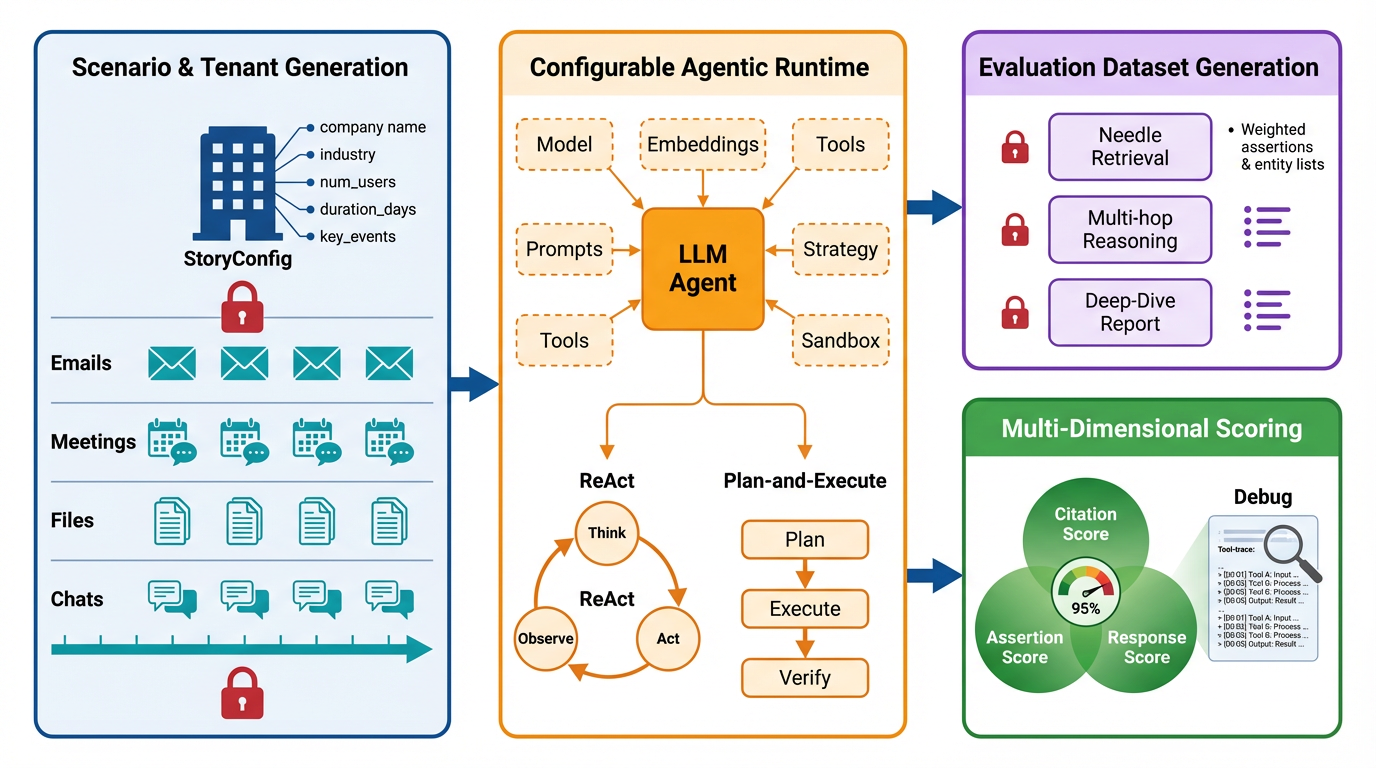
\includegraphics[width=0.9\textwidth]{figures/main_pipeline_research.png}
\caption{\textcolor{blue}{EABench graphical overview. The four coupled platform stages proceed from synthetic tenant generation (Stage~1), through configurable agent execution (Stage~2) and automated evaluation-dataset construction (Stage~3), to multi-dimensional scoring with interactive debugging (Stage~4), forming a single reproducible experimental pipeline.}}
\label{fig:graphical_abstract}
\end{figure}
\textcolor{blue}{Alongside these general-purpose efforts, enterprise-specific benchmarks---WebArena~\cite{zhou2023webarena}, AgentBench~\cite{liu2023agentbench}, ToolBench~\cite{qin2023toolllm}, WorkArena~\cite{drouin2024workarena}, EnterpriseBench~\cite{vishwakarma2025enterprisebench}, DRBench~\cite{abaskohi2025drbench}, and HERB~\cite{choubey2025benchmarking}---each capture important slices of agent capability, but they leave three recurring gaps for enterprise research. First, they generally rely on static datasets or fixed task pools, which prevents researchers from generating new organizational histories or stress-testing a method under controlled scenario variation; while dynamically generated benchmarks have been proposed~\cite{saxena2025continuous}, they address only narrow task domains and do not generalize to multi-source enterprise knowledge work. Second, they rarely expose the agent runtime and the judge as independently configurable objects, making systematic ablations across models, prompts, tools, embeddings, and scoring criteria unnecessarily expensive. Third, they under-specify the debugging problem: when an enterprise agent fails, researchers need to inspect the search trajectory, tool usage, citations, and permission context rather than only the final answer.}

\textcolor{blue}{EABench addresses these gaps through four tightly coupled contributions. The first contribution is a unified end-to-end platform that connects synthetic tenant generation, agent execution, and evaluation in a single reproducible pipeline. The second is extreme configurability: six major runtime dimensions---models, embeddings, cognitive architectures, prompts, tools, and sandbox implementations---are all hot-swappable without source-code edits. The third is configurable query generation and evaluation, in which the framework automatically generates three query types and pairs them with user-specific access context, ground-truth entity lists, weighted assertions, and judge prompts that can themselves be redefined without code changes. The fourth is scenario-aware enterprise simulation, which varies company size, industry, and event structure while supporting interactive debugging over the same runtime used for batch evaluation.}


\textcolor{blue}{This design changes the role of a benchmark from a fixed leaderboard to an experimental sandbox. A researcher can generate a legal-services tenant and a software-incident tenant from the same pipeline, evaluate ReAct and plan-and-execute agents under identical access constraints, swap only the embedding model or only the citation judge, and then inspect the full tool trace when performance changes. Table~\ref{tab:comparison} summarizes this shift relative to prior work.}





\textcolor{blue}{The rest of the paper develops these ideas in order. Section~\ref{sec:related} positions EABench relative to prior agent benchmarks and enterprise retrieval systems. Section~\ref{sec:method} formalizes the end-to-end platform architecture, the configurable runtime, the data-generation pipeline, the evaluation-dataset generator, the multi-dimensional evaluation harness, and the interactive debugging interface. Section~\ref{sec:scenarios} describes the scenario families used to instantiate the benchmark. Section~\ref{sec:experiments} specifies the experimental protocol supported by the framework, including cross-model evaluation, human validation, and ablation studies. Section~\ref{sec:conclusion} concludes with limitations and future directions.}


\begin{table}%[h]
\centering
\caption{\textcolor{blue}{Comparison of EABench with representative agent benchmarks. $\checkmark$ indicates direct support, Partial indicates limited or indirect support, and -- indicates that the capability is absent from the published benchmark design.}}
\label{tab:comparison}
\small
\resizebox{\linewidth}{!}{%
{\color{blue}
\begin{tabular}{p{3.8cm}cccccccc}
\toprule
\textbf{Feature} & \textbf{WebArena} & \textbf{AgentBench} & \textbf{ToolBench} & \textbf{WorkArena} & \textbf{DRBench} & \textbf{HERB} & \textbf{EnterpriseBench} & \textbf{EABench} \\
\midrule
End-to-end evaluation pipeline       & --            & --             & --             & --             & Partial        & Partial        & Partial        & $\checkmark$ \\
Configurable data generation          & --            & --             & --             & --             & Partial        & $\checkmark$   & Partial        & $\checkmark$ \\
Configurable agent runtime            & --            & --             & --             & --             & --             & --             & --             & $\checkmark$ \\
Configurable evaluation metrics       & --            & --             & --             & --             & Partial        & --             & --             & $\checkmark$ \\
Auto query + ground-truth generation  & --            & --             & --             & --             & --             & Partial        & Partial        & $\checkmark$ \\
Assertion-based fact checking         & --            & --             & --             & --             & Partial        & Partial        & --             & $\checkmark$ \\
User-level access control             & --            & --             & --             & Partial        & Partial        & Partial        & $\checkmark$   & $\checkmark$ \\
Interactive debugging                 & --            & --             & --             & --             & --             & --             & --             & $\checkmark$ \\
Pluggable LLM providers               & --            & Partial        & --             & --             & $\checkmark$   & $\checkmark$   & Partial        & $\checkmark$ \\
Sandboxed tool execution              & --            & Partial        & --             & --             & --             & --             & --             & $\checkmark$ \\
\bottomrule
\end{tabular}
}}% end color group, end resizebox
\end{table}


% ══════════════════════════════════════════════════════════════════════
% 2  RELATED WORK
% ══════════════════════════════════════════════════════════════════════
\section{Related Work}
\label{sec:related}

We review the literature across two primary axes: the evolution of agent benchmarking from general web environments to enterprise-specific tasks, and the enabling technologies behind EABench, including synthetic data generation, cognitive architectures, and automated evaluation metrics.

\subsection{Agent Benchmarks}

General-purpose benchmarks have been instrumental in driving rapid progress in LLM tool use. However, as discussed below, their reliance on static web environments and generic API puzzles limits their applicability to the messy, permission-gated reality of private organizational networks.

\textbf{WebArena}~\cite{zhou2023webarena} provides a realistic web browsing
environment with four web applications (shopping, reddit, GitLab, map) and 812
long-horizon tasks.  While WebArena evaluates task completion in a realistic
setting, its tasks are scoped to web interfaces and do not address enterprise
knowledge retrieval.  \textbf{WorkArena}~\cite{drouin2024workarena} extends
this approach to ServiceNow workflows, targeting enterprise service management
tasks.  However, its data is limited to a single application and does not cover
the richly inter-connected multi-source data of a real enterprise.

\textbf{AgentBench}~\cite{liu2023agentbench} is a multi-dimensional benchmark
spanning eight environments including OS, database, web browsing, and lateral
reasoning tasks.  It demonstrates that current LLMs struggle with multi-step
tool-use tasks; however, its environments are largely synthetic or game-like
rather than representative of knowledge-worker contexts.

\textbf{ToolBench}~\cite{qin2023toolllm} focuses specifically on evaluating
LLMs' ability to invoke real-world APIs from a large catalog of 16,000 APIs.
While this directly tests tool-use, the tasks are API-centric rather than
information-synthesis-centric, and there is no notion of user-level access
control or data provenance.

\textbf{$\tau$-bench}~\cite{yao2024taubench} introduces the concept of user
simulation for interactive task evaluation in airline and retail domains.  The
approach of simulating realistic user interactions---rather than specifying
fully deterministic tasks---is conceptually related to EABench's user-level
evaluation mode, though $\tau$-bench targets customer service scenarios rather
than enterprise knowledge work.

\textbf{Information Worker Benchmarks.} While systems such as \textbf{WorkArena}~\cite{drouin2024workarena} or OSWorld provide highly realistic tasks mapped to complex user interfaces, they remain fundamentally inflexible when modifications to the underlying environment or integrations of novel agent architectures are required. Conducting ablation studies within these robust ecosystems demands significant engineering overhead, restricting iterative cognitive architecture design.

\textbf{Static vs. Dynamic Environments.} \textbf{GAIA-2}~\cite{gaia2} and \textbf{SWE-Bench}~\cite{jimenez2024swebench} push the boundaries of general AI assistance by testing complex, real-world reasoning, multimodal tool use, and sophisticated software engineering tasks. However, these represent completely static and unalterable evaluation paradigms. Their rigid evaluation harnesses prevent isolating targeted variables---such as altering the underlying embedding model used in retrieval tools or limiting exposure to specific operational commands. Conversely, EABench explicitly addresses this via a deeply configurable design, granting researchers an open architectural playground to systematically investigate execution strategies across diverse scenario and runtime configurations.

  \subsection{Enterprise Agentic Benchmarks}
  
Recognizing the limitations of general domains, recent works have begun simulating enterprise environments. While these benchmarks test multi-hop reasoning over corporate artifacts, they often rely on fixed, non-extensible datasets, leaving a critical gap for highly configurable, generative sandboxes.
    
\textbf{DRBench}~\cite{abaskohi2025drbench} evaluates agents on open-ended, multi-hop deep research tasks that require synthesizing insight-driven reports from a mix of public web data and private company knowledge bases. Grounded in realistic user personas, DRBench spans a heterogeneous search space (including internal chats, cloud file systems, spreadsheets, and emails) and specifically scores an agent's ability to recall critical insights with proper source citations. 
    Similarly, \textbf{HERB}~\cite{choubey2025benchmarking} presents a benchmark containing 39,190 enterprise artifacts designed for evaluating deep search and retrieval-augmented generation over heterogeneous, interconnected data sources like documents, meeting transcripts, and Slack messages via synthetic workflows simulating product planning and support stages. While these benchmarks test multi-hop reasoning over enterprise artifacts, EABench distinguishes itself by generating a fully-coherent synthetic timeline, providing a fully configurable agent runtime (ReAct vs.\ Plan-and-Execute), and strictly verifying factuality via structural citation scoring combined with user-level access control.
Teams chats.  Its architecture involves retrieval-augmented generation (RAG)
over enterprise data with user-level access control.  While such systems
demonstrate the commercial viability of enterprise agents, they do not provide
open evaluation datasets or benchmarking infrastructure.

\textbf{Glean} and similar enterprise search platforms combine vector search
with access control lists (ACLs) to implement personalized search across
connected SaaS applications.  These systems illustrate the importance of
user-context-aware retrieval---a feature EABench explicitly supports through
its user-level indexing and filtering.

\subsection{Synthetic Data Generation for Benchmarks}

Real-world corporate data is scarce and constrained by extreme privacy bottlenecks. To overcome this, researchers have turned to LLM-driven synthetic generation. EABench extends these techniques beyond isolated QA pairs to construct fully interconnected, temporally coherent organizational ecosystems.

\textbf{AgentInstruct}~\cite{mitra2024agentinstruct} uses LLMs to generate
instruction tuning data by transforming raw documents through a pipeline of
multiple specialized agents.
\textbf{FrontierMath}~\cite{glazer2024frontiermath} demonstrates that
LLM-generated problems can challenge state-of-the-art models.
\textbf{WildChat}~\cite{zhao2024wildchat} collects naturally occurring LLM
conversations in the wild.

EABench's approach differs from prior work in that it generates
\emph{structured organizational corpora} rather than isolated question-answer
pairs.  The generator produces inter-connected narrative artifacts (emails,
meetings, files, chats) grounded in a shared storyline, enabling queries that
require multi-hop reasoning across document types and temporal reasoning over
event sequences.

\subsection{LLM-as-a-Judge Evaluation}

Evaluating open-ended, multi-step agent trajectories requires scalable metrics that transcend exact-string matching. LLM-as-a-Judge paradigms have emerged as a robust solution, which we adapt to perform granular citation verification and assertion checking while mitigating inherent evaluator biases.

Automated evaluation using LLMs as judges has gained significant traction following MT-Bench~\cite{zheng2023judging} and Chatbot Arena~\cite{chiang2024chatbot}. LLM judges show high correlation with human
preferences at lower cost and enable evaluation of open-ended responses that
resist automatic metrics.

EABench extends the LLM-as-a-Judge paradigm to \emph{agentic evaluation},
where the judge must assess not only the final response but also the
\emph{reasoning process}---including whether cited sources are accurate,
whether tool calls were appropriate, and whether the overall research plan was
followed.

\subsection{Cognitive Architectures and Agentic Workflows}

The cognitive architecture of an agent fundamentally dictates its capability and operational ceiling. Recent advancements have synthesized rigid chain-of-thought prompting into broader structured agentic workflows, which emphasize iterative refinement, dynamic tool use, and reflection over single-shot generation. Within this landscape, we contrast single-pass reasoning loops with deliberative planning and broader workflow frameworks, all of which EABench treats as first-class, easily configurable strategies for applied scientists.

The ReAct paradigm introduced the concept of interleaving reasoning traces with tool invocations~\cite{yao2022react}. This approach demonstrated that explicitly reasoning about the next action before taking it substantially improves task performance on knowledge-intensive tasks compared to standard zero-shot execution. Plan-and-Solve agents build upon and extend this fundamental idea by explicitly separating the planning phase, which handles the generation of a high-level task decomposition, from the execution phase~\cite{wang2023plansolve}. This deliberate separation can significantly improve reliability on complex multi-step tasks by preventing the underlying agent from losing the contextual thread during long and intricate tool-use sequences.

Furthermore, modern agentic workflows have evolved these frameworks by incorporating reflection, multi-turn tool calling, and structured orchestration. These workflows shift the paradigm from monolithic text generation to a composite system where an agent iteratively critiques its intrinsic execution trajectory, adapts to newly retrieved information, and dynamically alters its multi-step plan. EABench natively implements these advanced paradigms as first-class, configurable execution strategies. This deep integration systematically enables the direct comparison of performance characteristics across distinct cognitive architectures and iterative workflows directly within evaluation tasks.

\begin{figure}[t]
\centering
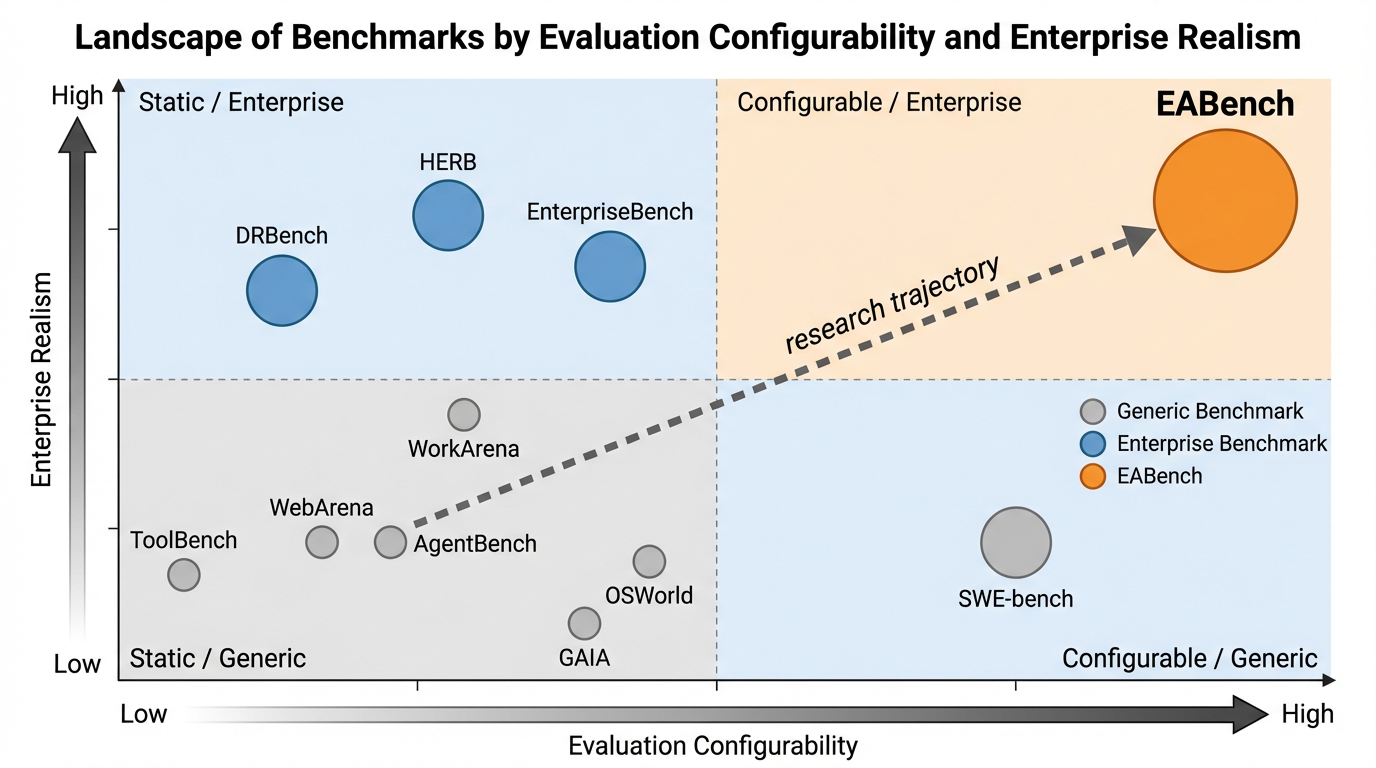
\includegraphics[width=0.9\textwidth]{figures/research_position.png}
%\fbox{\parbox{0.96\linewidth}{%
%\vspace{4pt}
%\small\color{blue}\itshape\raggedright
%\textbf{[Figure placeholder --- generation pending.]}
%A two-dimensional scatter-and-bubble chart.
%\textbf{X-axis:} ``Evaluation Configurability'' ranging from Low (left) to High (right).
%\textbf{Y-axis:} ``Enterprise Realism'' ranging from Low (bottom) to High (top).
%Four quadrant background fills with labels: bottom-left light gray (``Static / Generic''), bottom-right light blue (``Configurable / Generic''), top-left light blue (``Static / Enterprise''), top-right light orange (``Configurable / Enterprise'').
%Each benchmark is plotted as a labeled circle whose radius is proportional to the number of EABench feature rows (from Table~\ref{tab:comparison}) it satisfies.
%Approximate positions and sizes:
%WebArena (small, bottom-left);
%AgentBench (small, bottom-left, slightly right);
%ToolBench (small, far bottom-left);
%WorkArena (small, left-center);
%GAIA (small, bottom-center);
%OSWorld (small, bottom-center, above GAIA);
%SWE-bench (medium, bottom-right);
%DRBench (medium, top-left);
%HERB (medium, top-center-left);
%EnterpriseBench (medium, top-center, slightly right of HERB);
%EABench (large filled orange circle, top-right corner, labeled in bold, clearly in the ``Configurable / Enterprise'' quadrant).
%A dashed diagonal arrow from the WebArena cluster toward EABench annotated ``research trajectory.''
%Color scheme: generic benchmarks in gray; enterprise benchmarks in blue; EABench in orange; quadrant boundaries as thin dashed lines.
%\vspace{4pt}
%}}
\caption{\textcolor{blue}{Positioning of representative agent benchmarks along two axes: enterprise realism (y-axis) and evaluation configurability (x-axis). Bubble size reflects the number of first-class benchmark features supported (cf.\ Table~\ref{tab:comparison}). EABench uniquely occupies the top-right quadrant, combining scenario-aware organizational simulation with end-to-end configurability across all platform dimensions.}}
\label{fig:positioning}
\end{figure}

% ══════════════════════════════════════════════════════════════════════
% 3  METHODOLOGY
% ══════════════════════════════════════════════════════════════════════
\section{Methodology}
\label{sec:method}

\textcolor{blue}{We now describe the six components of the EABench platform in turn, covering the end-to-end architecture, the configurable runtime, the data-generation pipeline, the evaluation-dataset generator, the multi-dimensional evaluation harness, and the interactive debugging interface.}

\subsection{End-to-End Platform Architecture}
\label{sec:method_overview}

\textcolor{blue}{EABench is organized as a single experimental pipeline rather than a loose collection of scripts. A scenario specification begins with a \texttt{StoryConfig}, which defines the company profile, timeline, employee count, and key events that drive narrative evolution. The tenant generator expands this specification into a multi-modal enterprise corpus containing users, emails, chats, meetings, and files. The same tenant is then consumed by the agent runtime, which executes under a concrete user identity and records its full tool trajectory. Finally, the evaluation harness scores the resulting answer with both deterministic and judge-based metrics. Because each stage writes explicit artifacts to disk, the entire process is reproducible and inspectable.}

\begin{figure}[h]
\centering
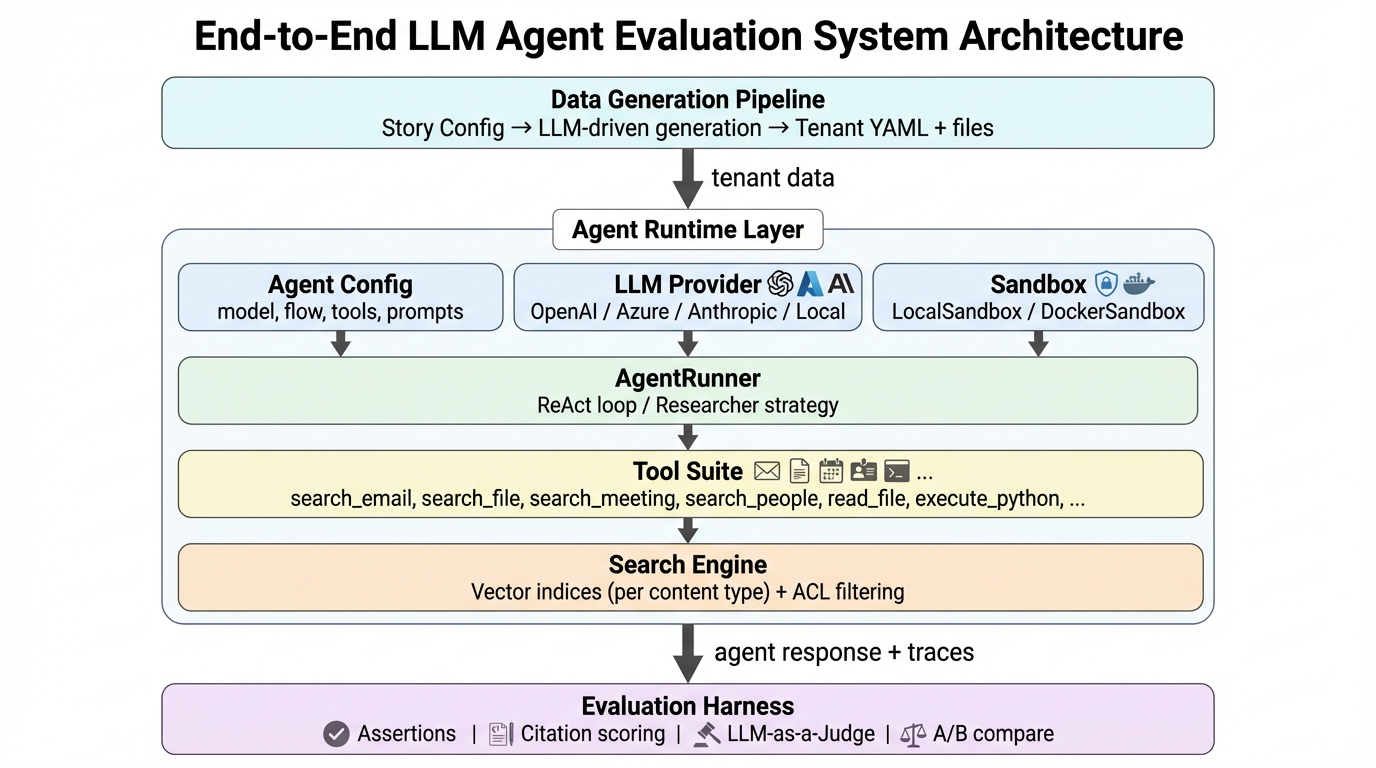
\includegraphics[width=0.85\textwidth]{figures/agent-evaluator-framework.png}
%\resizebox{0.96\linewidth}{!}{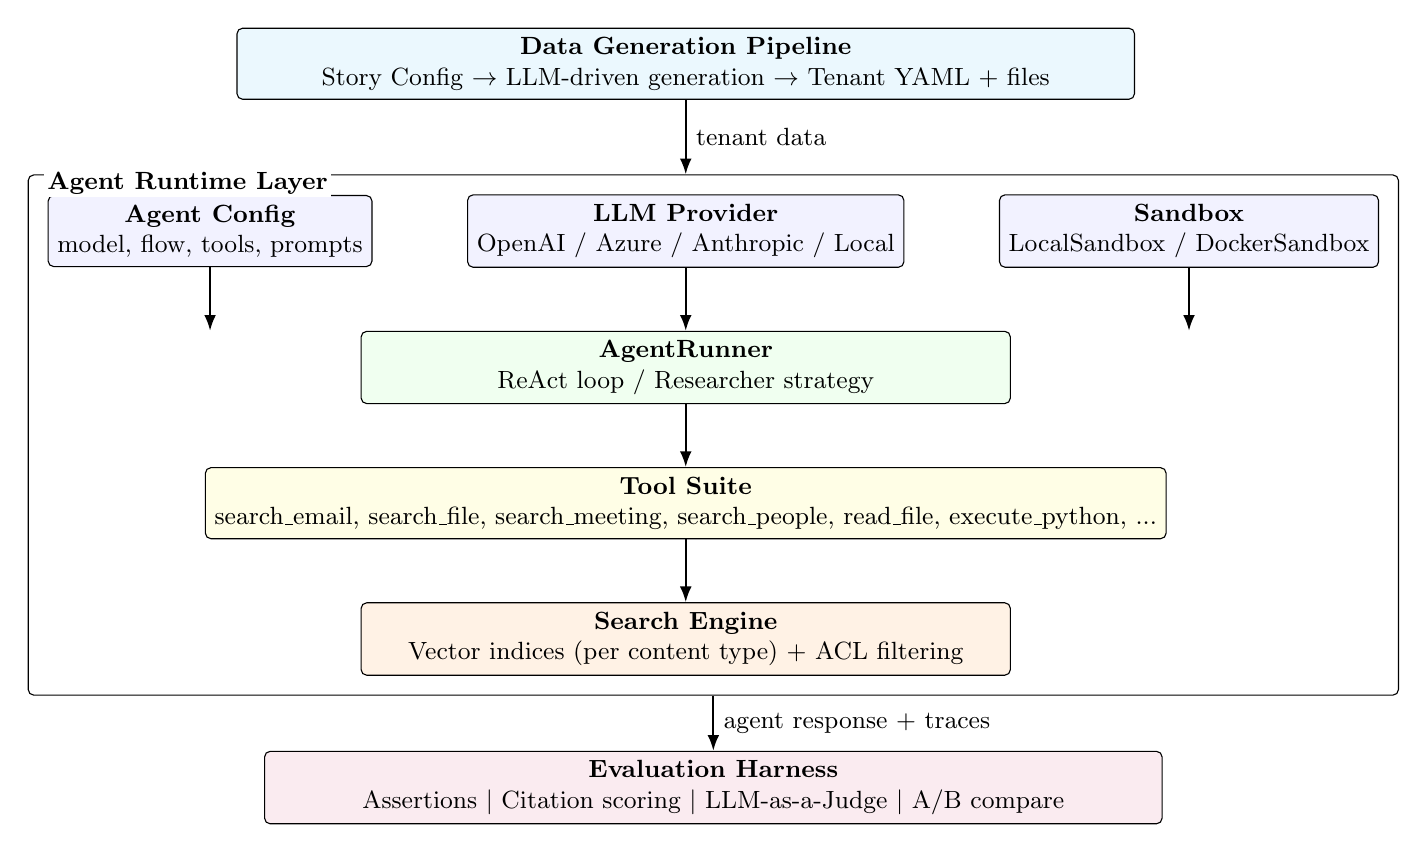
\begin{tikzpicture}[
  font=\small,
  box/.style={draw, rounded corners=2pt, align=center, minimum height=8mm},
  outer/.style={draw, rounded corners=2pt, inner sep=7pt},
  arr/.style={-{Latex[length=2mm]}, thick}
]
  % Top pipeline
  \node[box, fill=cyan!8, minimum width=0.94\textwidth] (datagen) {
    \textbf{Data Generation Pipeline}\\
    Story Config $\rightarrow$ LLM-driven generation $\rightarrow$ Tenant YAML + files
  };

  % Runtime top row (symmetric around center)
  \node[box, fill=blue!5, minimum width=0.20\textwidth, below=12mm of datagen] (llmprov) {
    \textbf{LLM Provider}\\
    OpenAI / Azure / Anthropic / Local
  };
  \node[box, fill=blue!5, minimum width=0.20\textwidth, left=12mm of llmprov] (agentcfg) {
    \textbf{Agent Config}\\
    model, flow, tools, prompts
  };
  \node[box, fill=blue!5, minimum width=0.20\textwidth, right=12mm of llmprov] (sandbox) {
    \textbf{Sandbox}\\
    LocalSandbox / DockerSandbox
  };

  % Runtime stack
  \node[box, fill=green!6, minimum width=0.68\textwidth, below=8mm of llmprov] (runner) {
    \textbf{AgentRunner}\\
    ReAct loop / Researcher strategy
  };

  \node[box, fill=yellow!10, minimum width=0.68\textwidth, below=8mm of runner] (tools) {
    \textbf{Tool Suite}\\
    search\_email, search\_file, search\_meeting, search\_people, read\_file, execute\_python, ...
  };

  \node[box, fill=orange!10, minimum width=0.68\textwidth, below=8mm of tools] (search) {
    \textbf{Search Engine}\\
    Vector indices (per content type) + ACL filtering
  };

  % Runtime container and title
  \node[outer, fit=(agentcfg)(llmprov)(sandbox)(runner)(tools)(search)] (runtime) {};
  \node[anchor=north west, fill=white, inner sep=1.2pt, font=\bfseries\small]
    at ([xshift=2mm,yshift=0.8mm]runtime.north west) {Agent Runtime Layer};

  % Bottom evaluation
  \node[box, fill=purple!8, minimum width=0.94\textwidth, below=7mm of runtime] (eval) {
    \textbf{Evaluation Harness}\\
    Assertions $\mid$ Citation scoring $\mid$ LLM-as-a-Judge $\mid$ A/B compare
  };

  % Orthogonal flows
  \draw[arr] (datagen.south) -- node[right]{\small tenant data} (datagen.south |- runtime.north);
  \draw[arr] (agentcfg.south) -- (agentcfg.south |- runner.north);
  \draw[arr] (llmprov.south) -- (runner.north);
  \draw[arr] (sandbox.south) -- (sandbox.south |- runner.north);
  \draw[arr] (runner.south) -- (tools.north);
  \draw[arr] (tools.south) -- (search.north);
  \draw[arr] (runtime.south) -- node[right]{\small agent response + traces} (runtime.south |- eval.north);
\end{tikzpicture}
}
\caption{\textcolor{blue}{End-to-end EABench architecture. The platform connects scenario specification, tenant generation, configurable runtime execution, evaluation-case generation, and interactive debugging in one reproducible workflow.}}
\label{fig:arch}
\end{figure}

\textcolor{blue}{This architecture supports two complementary use modes. In batch mode, researchers generate a tenant, evaluate one or more agent configurations, and compare the resulting metric distributions. In interactive mode, they run the same runtime against the same tenant but inspect intermediate search results, tool calls, citations, and user context while debugging failure cases. The shared backend is important: debugging traces come from the exact runtime that produces benchmark results, so qualitative inspection and quantitative evaluation remain aligned.}

\begin{table}[h]
\centering
\caption{\textcolor{blue}{Primary artifacts exchanged across the EABench pipeline.}}
\label{tab:pipeline_artifacts}
\small
{\color{blue}
\begin{tabular}{p{0.17\linewidth}p{0.24\linewidth}p{0.48\linewidth}}
\toprule
\textbf{Stage} & \textbf{Primary artifact} & \textbf{Role in the pipeline} \\
\midrule
Scenario specification & \texttt{StoryConfig} and prompt templates & Defines the enterprise domain, timeline, narrative drivers, and generator behavior \\
Tenant generation & \texttt{tenant.yaml}, \texttt{generation\_log.json}, modality-specific YAML files, sandbox files & Materializes a coherent enterprise workspace with explicit provenance \\
Evaluation dataset generation & \texttt{eval\_dataset\_*.yaml} & Converts raw tenant history into query cases with \texttt{user\_id}, \texttt{entity\_list}, and weighted assertions \\
Agent runtime & Response text, tool traces, token and latency metrics & Executes a concrete agent configuration under a specific access context \\
Evaluation harness & Per-case JSON results and aggregate summaries & Produces assertion, citation, and operational diagnostics for comparison and analysis \\
Interactive debugging & Search evidence, tool-call logs, citation traces & Explains success and failure modes on individual cases without changing the runtime \\
\bottomrule
\end{tabular}
}
\end{table}

\textcolor{blue}{The key systems claim of EABench is therefore not only that each subsystem is configurable, but that the interfaces between subsystems are stable and explicit. A change in the generator alters the tenant and the resulting query set; a change in the runtime alters the trajectory and answer; a change in the judge alters the scoring layer. By exposing these seams directly, EABench makes causal experimentation possible.}
\subsection{Configurable Agentic Runtime}
\label{sec:method_runtime}

\subsubsection{YAML Configuration Schema}

The runtime follows a configuration-as-code model in which each agent variant is represented by a single YAML file. This file specifies the reasoning model, embedding model, system prompt, optional planning prompt, per-tool query-analyzer prompts, tool exposure, and flow strategy. The design choice is deliberate: researchers should be able to version-control an agent definition, rerun it on a new tenant, and attribute behavioral changes to the configuration diff rather than to hidden code edits.

\begin{figure}[t]
\centering
\begin{minipage}{0.92\linewidth}
\begin{lstlisting}[basicstyle=\color{blue}\small\ttfamily]
id: react-agent-v1
version: "1.0.0"
model:
  provider: azure
  name: gpt-4o
  parameters: {temperature: 0.7}
embedding:
  provider: azure
  model: text-embedding-ada-002
system_prompt: |
  You are an intelligent enterprise assistant.
  {user_profile}
query_analyzer_prompt:
  search_email: |
    Analyze the user's email query and return
    strategy, refined_query, and sender_name.
tools:
  definitions:
    - search_email
    - search_file
    - search_meeting
    - search_people
    - read_file
    - execute_python
flow:
  strategy: react
  max_turns: 5
\end{lstlisting}
\end{minipage}
\caption{Condensed runtime configuration illustrating how model choice, prompt behavior, tool exposure, and flow strategy are all declared in YAML.}
\label{lst:runtime_yaml}
\end{figure}

\begin{table}[h]
\centering
\caption{Six runtime dimensions that can be changed without source-code edits.}
\label{tab:runtime_dimensions}
\small
\begin{tabular}{p{0.17\linewidth}p{0.24\linewidth}p{0.48\linewidth}}
\toprule
\textbf{Dimension} & \textbf{Configuration field} & \textbf{Research question enabled} \\
\midrule
Reasoning model & \texttt{model.*} & How sensitive is performance to the underlying LLM family and decoding parameters? \\
Embedding model & \texttt{embedding.*} & How much of end-to-end performance is driven by retrieval quality rather than reasoning quality? \\
Cognitive architecture & \texttt{flow.strategy} & Does ReAct or plan-and-execute better handle multi-step enterprise tasks? \\
Global prompting & \texttt{system\_prompt}, \texttt{planning\_prompt} & How do role instructions and planning structure affect behavior and citation quality? \\
Tool exposure & \texttt{tools.definitions} & Which tools are necessary for each query type, and what are the failure modes when they are removed? \\
Sandbox implementation & tool dependencies and runtime backend & How do local, remote, or more restrictive execution environments change tool use? \\
\bottomrule
\end{tabular}

\end{table}

\subsubsection{Cognitive Architectures}

EABench currently exposes two cognitive architectures. Under the \texttt{react} strategy, the runtime loops through thought, tool call, observation, and response generation until the model emits a final answer or reaches a hard turn limit. Under the \texttt{researcher} strategy, the runtime first invokes a planner to produce a structured plan and then executes that plan with the normal tool-enabled loop. The second strategy adds overhead, but it is often better suited to multi-hop cases in which the agent must identify a dependency chain before any single tool call is obviously useful.

\begin{table}[t]
\centering
\caption{Comparison of the two built-in runtime strategies.}
\label{tab:strategy_compare}
\small
\begin{tabular}{p{0.16\linewidth}p{0.18\linewidth}p{0.18\linewidth}p{0.30\linewidth}}
\toprule
\textbf{Strategy} & \textbf{First action} & \textbf{Typical strength} & \textbf{Typical failure mode} \\
\midrule
ReAct & Immediate tool-enabled reasoning & Fast response on local retrieval tasks & Can drift on long dependency chains or overlook needed decomposition \\
Researcher & Tool-free planning pass & Stronger structure on multi-step tasks & Higher token usage and possible over-planning on simple cases \\
\bottomrule
\end{tabular}

\end{table}

\begin{figure}[t]
\centering
%\fbox{\parbox{0.96\linewidth}{%
%\vspace{4pt}
%\small\color{blue}\itshape\raggedright
%\textbf{[Figure placeholder --- generation pending.]}
%A side-by-side two-panel comparison diagram separated by a vertical dashed center line, with a shared header banner.
%\textbf{Header banner (spanning both panels):} A YAML code snippet showing \texttt{flow.strategy: react} (left half) and \texttt{flow.strategy: researcher} (right half), with bold label above: ``EABench-configurable strategy selection (single YAML field).''
%\textbf{Left panel --- ReAct:}
%Vertical stack of rounded boxes connected by solid downward arrows:
%(1)~``User Query'' box (deep blue, top);
%(2)~``Reasoning'' box (amber) annotated with a thought-bubble: ``Which tool is needed and why?'';
%(3)~``Action'' box (orange) showing a tool-call icon with parameter fields;
%(4)~``Observation'' box (teal) showing a tool-result snippet.
%A curved dashed arrow on the left side of the stack loops from the Observation box back up to the Reasoning box, labeled ``repeat until answer ready.''
%A final ``Answer'' box (green) sits below Observation after the loop terminates, connected by a solid arrow.
%\textbf{Right panel --- Plan-and-Execute:}
%Two vertically stacked phases with a horizontal divider:
%\textit{Phase~1 ``Plan''}: A ``Planner LLM'' box (deep blue) outputs a numbered clipboard: Step~1, Step~2, \ldots, Step~N.
%A thick downward arrow labeled ``hand off complete plan'' leads to:
%\textit{Phase~2 ``Execute''}: An ``Executor'' rounded rectangle (orange) that loops through each step, showing \textit{(Step $i$)} $\rightarrow$ Tool Call (orange) $\rightarrow$ Observation (teal) for each step, with a small inner circular arrow labeled ``steps~1\ldots N.''
%A ``Final Answer'' box (green) sits below the executor after all steps complete.
%\textbf{Annotation differences:} The ReAct panel is narrower and denser; the Plan-and-Execute panel is taller with a clear two-phase separation.
%Color scheme: query/answer boxes in deep blue and green; reasoning/planning in amber; action/execution in orange; observations in teal; dashed loop arrows in gray.
%\vspace{4pt}
%}}
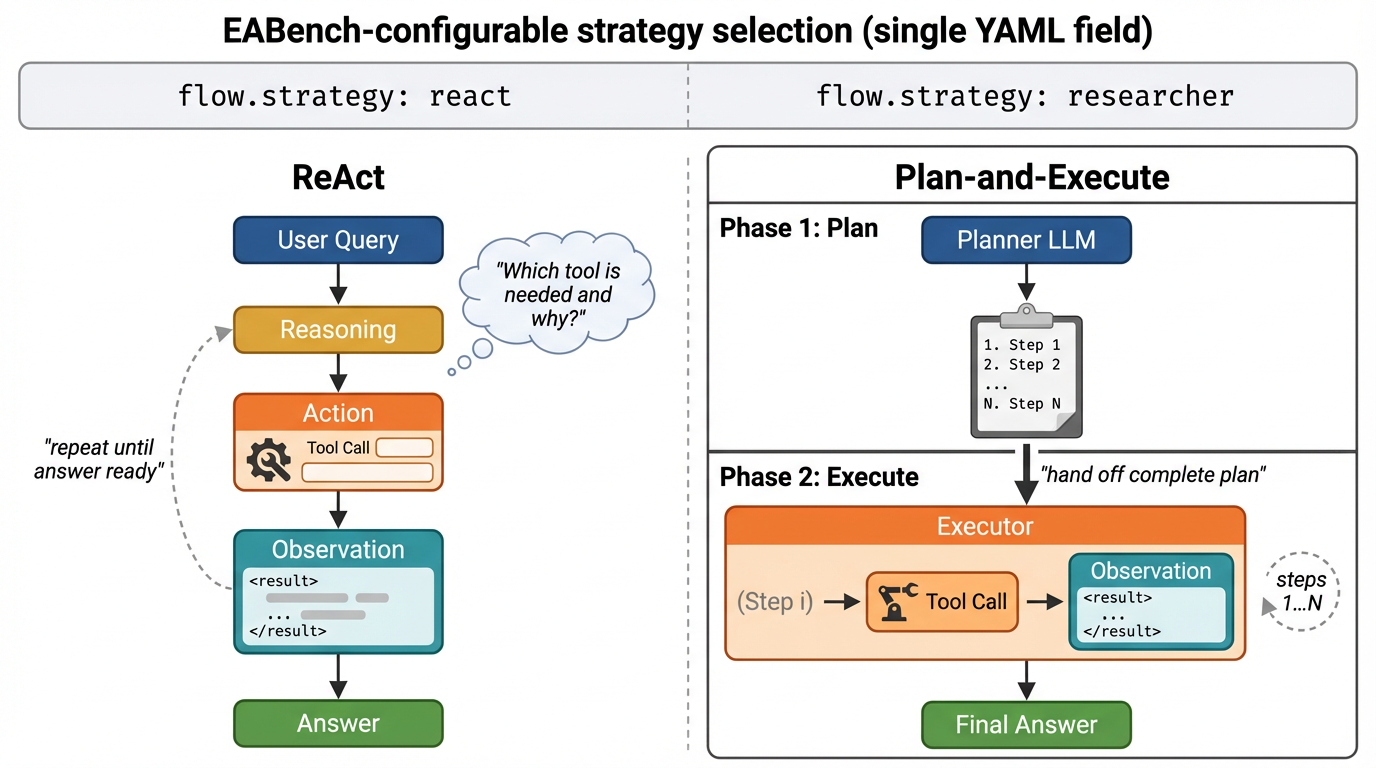
\includegraphics[width=0.9\textwidth]{figures/agent-architecture-config.png}
\caption{The two cognitive architectures natively supported by EABench as hot-swappable \texttt{flow.strategy} values. ReAct (left) interleaves reasoning and acting in a tight feedback loop; Plan-and-Execute (right) separates a global planning phase from sequential step-wise execution, reducing context drift on long multi-hop tasks.}
\label{fig:cognitive_arch}
\end{figure}

\subsubsection{Multi-Provider LLM Support}

The runtime separates the configuration schema from the provider implementation through a common LLM interface. Provider choice is driven by the YAML field \texttt{model.provider}, while credentials and deployment-specific settings are resolved from environment variables. This separation makes provider swapping operationally cheap: researchers can move between OpenAI, Azure-hosted deployments, or compatible local endpoints while preserving the rest of the runtime definition. That property is especially important for cross-model evaluations, because it prevents provider migration from becoming a hidden code change.

\subsubsection{Enterprise Tool Suite and Search Infrastructure}

The built-in tool suite combines semantic retrieval tools with sandboxed execution tools. Search tools cover emails, files, meetings, people, one-to-one chats, group chats, and channel messages. Execution tools cover file inspection, directory listing, shell execution, and Python execution. Tools are registered through a decorator-based registry that automatically exports JSON schemas for model-facing tool calling, while dependencies such as the sandbox, search engine, and query analyzer are injected by the runner. This keeps tool implementations modular and makes tool ablations straightforward: removing a tool from the YAML file is sufficient to change the agent's action space.

Retrieval itself is implemented as a set of separate vector indices rather than as one monolithic store. EABench indexes at least nine content collections, including file snippets, full file contents, emails, chats, group chats, channels, meeting metadata, meeting transcripts, and user profiles. Similarity is computed with cosine similarity, and the resulting embeddings are cached on disk to avoid recomputation across repeated evaluations. The indices are filtered by user context before results are returned, which means the runtime and the evaluator both observe the same access-controlled search space.

\subsubsection{Query Analyzer}

An optional LLM-driven query analyzer sits between the user request and the retrieval tools. Instead of forwarding raw language directly to the vector index, the analyzer can refine a query, select a search strategy, or resolve a sender filter before retrieval occurs. Because its prompts are themselves configurable in YAML, EABench treats search refinement as a first-class experimental variable. Researchers can therefore study not only whether a search tool is useful, but whether specific decomposition heuristics or query rewrites materially improve retrieval fidelity.
\subsection{Scenario-Aware Synthetic Data Generation}
\label{sec:method_generation}

\subsubsection{StoryConfig and Scenario Specification}

Synthetic tenant generation begins with a \texttt{StoryConfig} that defines the company profile and the narrative arc the generator must realize. The configuration includes the company name, industry, company size, number of users, duration of the simulation, and a list of key events that anchor the narrative. This representation is compact enough for rapid scenario design yet expressive enough to vary organizational complexity and event density. The same generator can therefore instantiate a university administration scenario, a legal-services scenario, or a software-incident scenario without changing the code path.

\begin{table}[t]
\centering
\caption{Core fields in the \texttt{StoryConfig} specification.}
\label{tab:storyconfig_fields}
\small
\begin{tabular}{p{0.22\linewidth}p{0.14\linewidth}p{0.52\linewidth}}
\toprule
\textbf{Field} & \textbf{Type} & \textbf{Purpose} \\
\midrule
\texttt{company\_name} & string & Names the tenant and appears in prompts and output paths \\
\texttt{industry} & string & Conditions vocabulary, artifacts, and domain-specific events \\
\texttt{company\_size} & string & Influences organizational breadth and communication patterns \\
\texttt{num\_users} & int & Sets the size of the user roster and social graph \\
\texttt{duration\_days} & int & Controls the temporal window over which history accumulates \\
\texttt{key\_events} & list[string] & Defines narrative milestones that should recur across modalities \\
\texttt{description} & string & Supplies free-form scenario context to the generator prompts \\
\bottomrule
\end{tabular}

\end{table}

\subsubsection{Five-Stage Generation Pipeline}

The generator executes in five stages. It first creates the directory scaffold and initializes modality-specific YAML files. It then generates the user roster in batches, using diversity prompts to avoid name collisions and departmental imbalance. Next, it iterates day by day through the simulation, producing 3--5 narrative events per day while maintaining rolling history buffers. It materializes those events as emails, chats, meetings, and files, and it finally writes a complete \texttt{generation\_log.json} that serves as the source material for evaluation-case generation. The pipeline is incremental by design: artifacts are appended to disk as they are generated, which supports large tenants without requiring all content to remain in memory.

\begin{table}[h]
\centering
\caption{Five-stage tenant-generation process.}
\label{tab:generation_pipeline}
\small
\begin{tabular}{p{0.07\linewidth}p{0.22\linewidth}p{0.60\linewidth}}
\toprule
\textbf{Stage} & \textbf{Name} & \textbf{Output and purpose} \\
\midrule
1 & Directory scaffold and initialization & Creates tenant directories, empty modality YAML files, and a persistent workspace for generated documents \\
2 & User generation with diversity control & Produces the employee roster, titles, departments, managers, skills, and group memberships while avoiding duplicates \\
3 & Daily narrative generation & Expands key events into day-level story beats using recent-history and long-history buffers to preserve temporal coherence \\
4 & Artifact materialization and cross-referencing & Generates emails, chats, meetings, and files whose content explicitly references shared events and decisions \\
5 & Evaluation-log export & Serializes the full event history into \texttt{generation\_log.json} for downstream query generation and auditability \\
\bottomrule
\end{tabular}

\end{table}

\subsubsection{Content Type Generation}

Each artifact type is generated with a schema tailored to its role in enterprise communication. Emails are produced in two steps: a summary pass proposes sender, recipients, subject, and context, and a second pass expands that summary into realistic prose. Chats are likewise generated from conversation summaries into timestamped message sequences. Meetings produce three linked artifacts: metadata, transcript, and sidebar chat. Files are created as both metadata entries and concrete documents inside the sandboxed file tree. This staged process gives the generator enough structure to maintain consistency while still allowing varied surface realizations.

\subsubsection{Narrative Coherence Mechanisms}

Long-range coherence is preserved through explicit memory structures rather than through prompt length alone. A recent-history buffer stores the last several days of events verbatim, while a long-history buffer stores compressed summaries of earlier periods. Every seven simulated days, the recent buffer is summarized and appended to the long-term history. This mechanism allows later generations to mention prior incidents, decisions, and unresolved tensions without forcing the model to ingest the entire raw history each day. Cross-document references are then encouraged directly in the prompts, so that an email can cite a meeting outcome, a file can summarize a discussion from chat, and a report can reference both.

\begin{figure}[h]
\centering
%\fbox{\parbox{0.96\linewidth}{%
%\vspace{4pt}
%\small\color{blue}\itshape\raggedright
%\textbf{[Figure placeholder --- generation pending.]}
%A directed graph illustrating synthetic artifact creation and inter-document linkage within a single generated tenant.
%\textbf{Top-center node:} A dark-blue rounded rectangle labeled ``StoryConfig'' with five child annotation labels fanning out: company name, industry, num\_users, duration\_days, key\_events.
%\textbf{Below StoryConfig:} A horizontal five-stage chevron pipeline strip (Stage~1:~Directory Scaffold $\rightarrow$ Stage~2:~User Generation $\rightarrow$ Stage~3:~Daily Narrative $\rightarrow$ Stage~4:~Artifact Materialization $\rightarrow$ Stage~5:~Log Export), styled with left-pointing chevron shapes in mid-blue tones. A downward arrow from StoryConfig enters Stage~1.
%\textbf{Below the pipeline strip:} Four vertical artifact ``lanes'' separated by thin gray dividers (left to right):
%\textit{Lane~1 (Emails, blue-teal)}: A stack of four envelope icons at timestamps Day~1, Day~3, Day~7, Day\ldots, connected by thin timeline arrows.
%\textit{Lane~2 (Meetings, teal)}: Calendar+speech-bubble icons at Day~2, Day~5, Day~9.
%\textit{Lane~3 (Files, teal-green)}: Document icons at Day~4, Day~8.
%\textit{Lane~4 (Chats, green)}: Speech-bubble chain icons at Day~1, Day~3, Day~6, Day~10.
%\textbf{Cross-lane dashed red arrows} showing inter-artifact references (labeled):
%``references person'' (Email Day~3 $\rightarrow$ User node);
%``cites file'' (Meeting Day~5 $\rightarrow$ File Day~4);
%``follows up on meeting'' (Chat Day~6 $\rightarrow$ Meeting Day~5);
%``triggered by email'' (File Day~8 $\leftarrow$ Email Day~7).
%These cross-lane arrows represent the dependency links that enable multi-hop reasoning queries.
%\textbf{Bottom:} A horizontal shared timeline bar spanning all four lanes, labeled ``Simulated timeline (Day~1 \ldots Day~$N$)'' with evenly spaced tick marks.
%Below the timeline, two overlapping buffer icons: ``Recent-history buffer (last $k$ days verbatim)'' and ``Long-history buffer (compressed summaries)'' connected by a ``summarize every 7 days'' arrow.
%Color scheme: StoryConfig box and pipeline chevrons in deep blue; lane icons in teal-to-green gradient; cross-lane arrows in crimson; timeline bar in medium gray; buffer icons in light blue.
%\vspace{4pt}
%}}
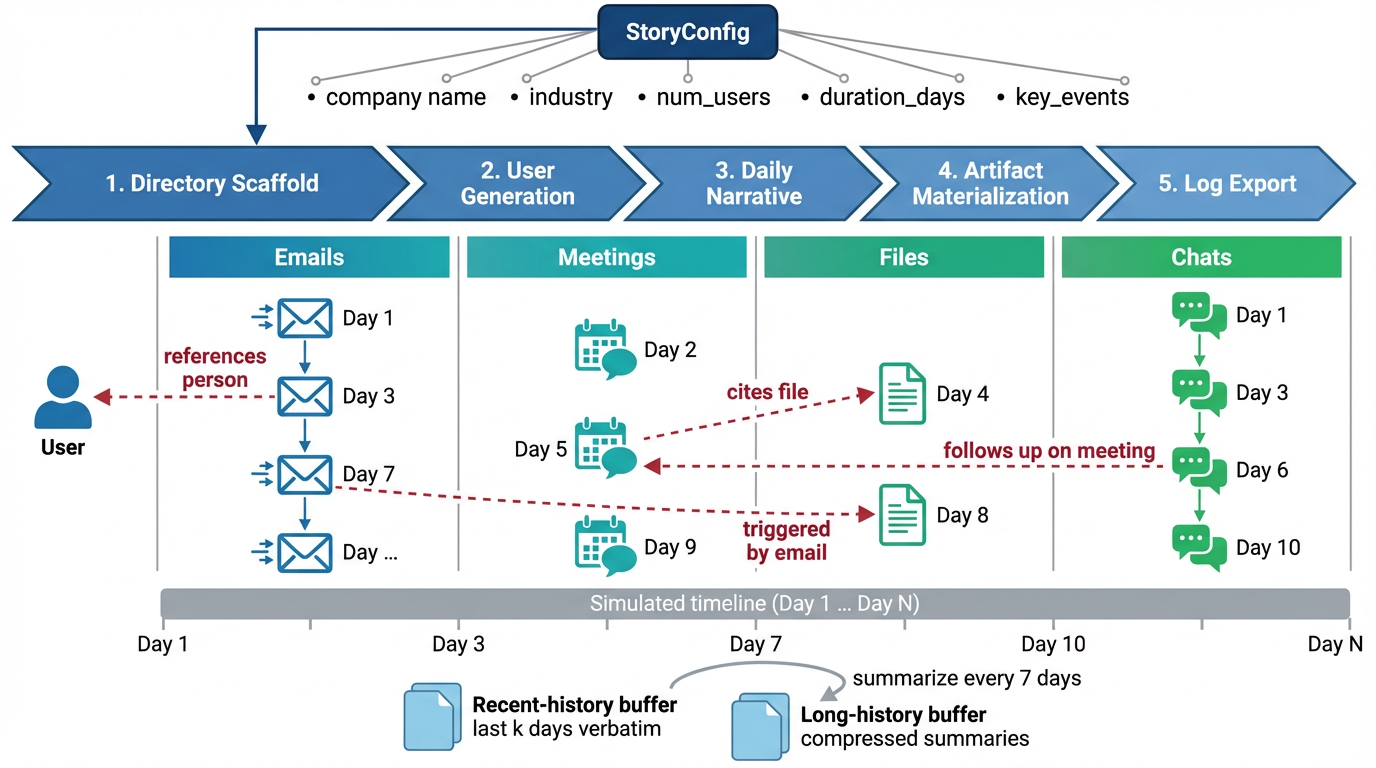
\includegraphics[width=0.9\textwidth]{figures/tenant-generation-pipeline.png}
\caption{EABench five-stage tenant-generation pipeline and inter-artifact linkage graph. A single \texttt{StoryConfig} drives the parallel creation of emails, meetings, files, and chats, which are connected by explicit cross-document references along a shared temporal timeline. These cross-references are what enable multi-hop and temporal reasoning evaluation cases.}
\label{fig:data_generation}
\end{figure}
\subsection{Configurable Evaluation Dataset Generation}
\label{sec:method_evaldataset}

\subsubsection{Three Query Types}

\textcolor{blue}{EABench does not treat evaluation cases as fixed annotations authored by hand. Instead, it derives them automatically from the generated tenant history, producing three query types that cover retrieval, reasoning, and synthesis. Needle-in-a-haystack cases ask the agent to locate a specific artifact or a very small set of artifacts without ever naming internal identifiers explicitly. Multi-step reasoning cases require the agent to follow a dependency chain across multiple modalities, such as resolving a person in one artifact and then using that reference to locate the decisive meeting or file. Deep-dive report cases ask for a coherent summary of an incident or initiative spread across several days of activity. This tripartite design ensures that evaluation does not collapse to a single notion of success.}

\begin{figure}[t]
\centering
%\resizebox{0.95\linewidth}{!}{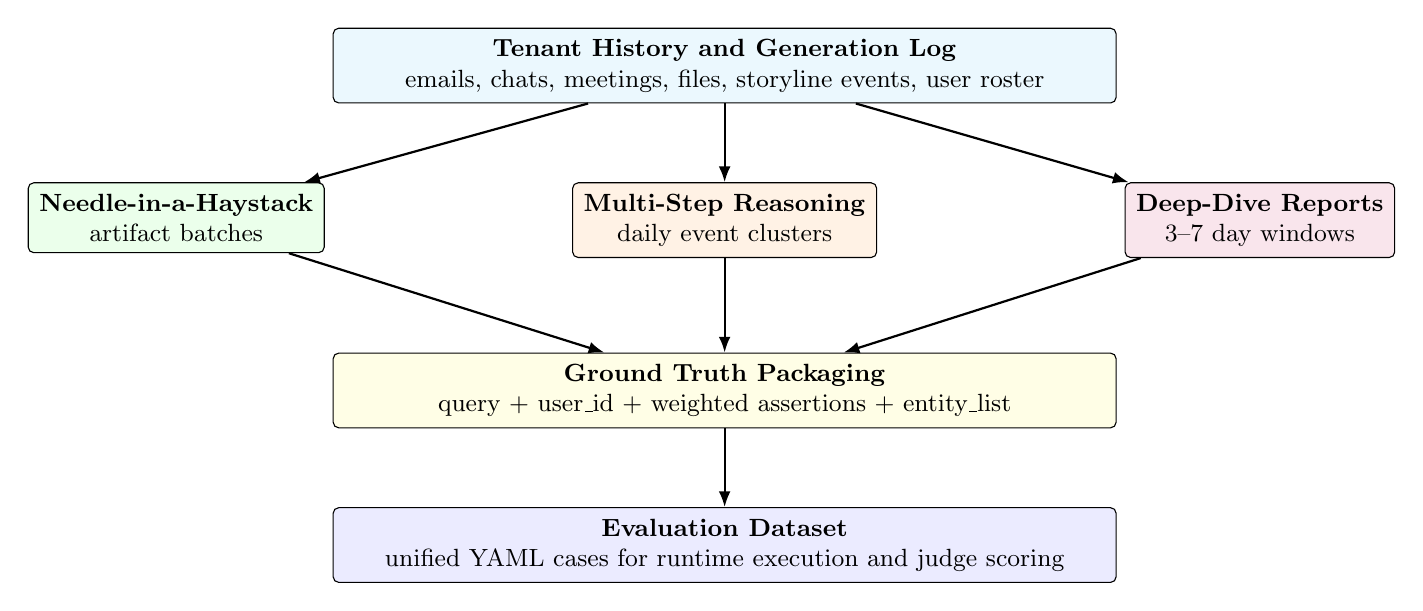
\begin{tikzpicture}[
  font=\small,
  box/.style={draw, rounded corners=2pt, align=center, minimum height=8mm, inner sep=4pt},
  arr/.style={-{Latex[length=2mm]}, thick}
]
  \node[box, fill=cyan!8, minimum width=0.82\linewidth] (log) {
    \textbf{Tenant History and Generation Log}\\
    emails, chats, meetings, files, storyline events, user roster
  };

  \node[box, fill=green!8, minimum width=0.24\linewidth, below left=10mm and 1mm of log] (search) {
    \textbf{Needle-in-a-Haystack}\\
    artifact batches
  };
  \node[box, fill=orange!10, minimum width=0.24\linewidth, below=10mm of log] (multihop) {
    \textbf{Multi-Step Reasoning}\\
    daily event clusters
  };
  \node[box, fill=purple!10, minimum width=0.24\linewidth, below right=10mm and 1mm of log] (report) {
    \textbf{Deep-Dive Reports}\\
    3--7 day windows
  };

  \node[box, fill=yellow!10, minimum width=0.82\linewidth, below=12mm of multihop] (gt) {
    \textbf{Ground Truth Packaging}\\
    query + user\_id + weighted assertions + entity\_list
  };

  \node[box, fill=blue!8, minimum width=0.82\linewidth, below=10mm of gt] (dataset) {
    \textbf{Evaluation Dataset}\\
    unified YAML cases for runtime execution and judge scoring
  };

  \draw[arr] (log) -- (search);
  \draw[arr] (log) -- (multihop);
  \draw[arr] (log) -- (report);
  \draw[arr] (search) -- (gt);
  \draw[arr] (multihop) -- (gt);
  \draw[arr] (report) -- (gt);
  \draw[arr] (gt) -- (dataset);
\end{tikzpicture}}
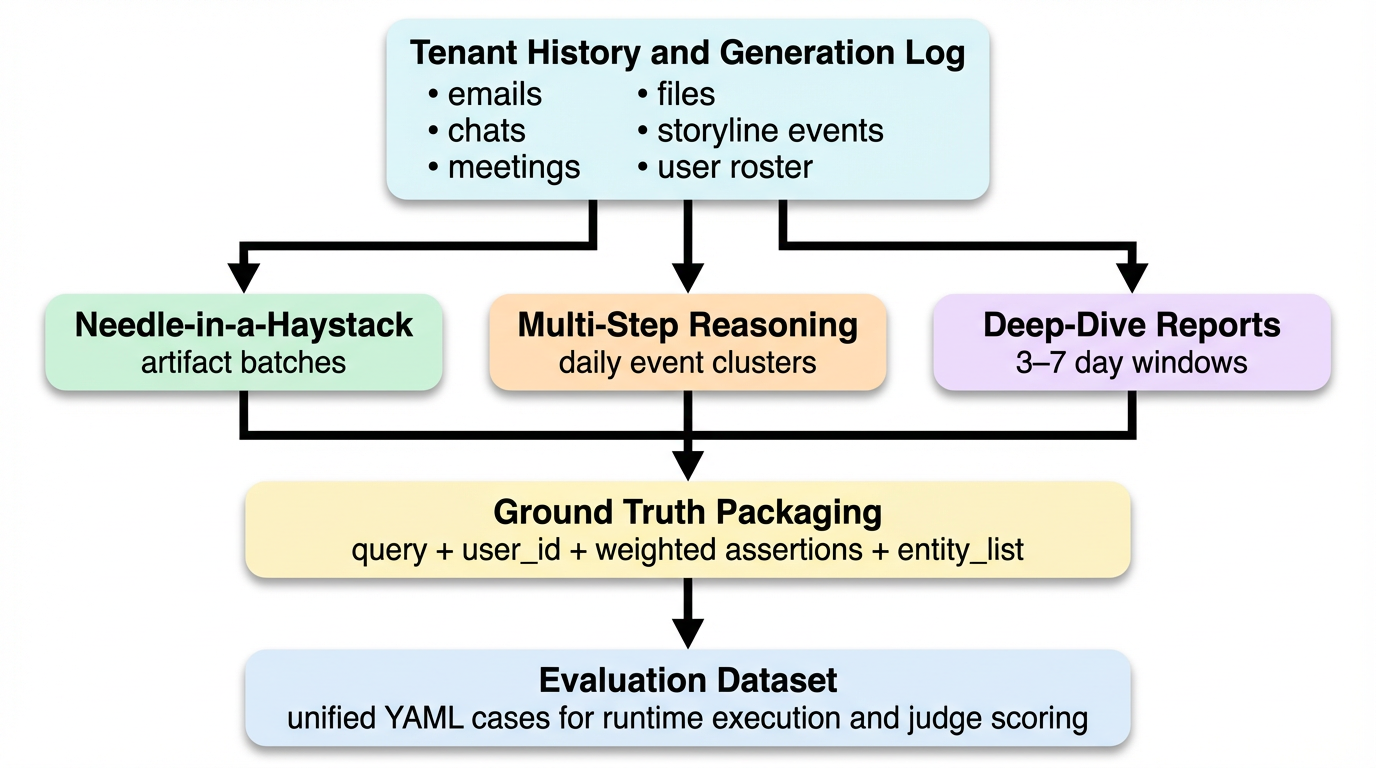
\includegraphics[width=0.7\textwidth]{figures/eval_data_generation_pipeline.png}
\caption{\textcolor{blue}{Evaluation-case generation pipeline. The same tenant history is re-sliced into retrieval, reasoning, and report-generation cases, each with explicit user context and ground truth.}}
\label{fig:eval_pipeline}
\end{figure}

\begin{table}[h]
\centering
\caption{\textcolor{blue}{Automatically generated query types in EABench.}}
\label{tab:query_types}
\small
{\color{blue}
\begin{tabular}{p{0.21\linewidth}p{0.34\linewidth}p{0.35\linewidth}}
\toprule
\textbf{Query type} & \textbf{Typical form} & \textbf{Primary benchmarked capability} \\
\midrule
Needle-in-a-haystack retrieval & Request to find a specific email, file, meeting, or message using natural constraints such as date, author, topic, or artifact type & Precision retrieval under realistic phrasing and user-level access control \\
Multi-step reasoning & Request whose answer depends on chaining evidence across multiple artifacts, often across different modalities & Decomposition, dependency tracking, and selective tool use \\
Deep-dive report generation & Request for a briefing, incident summary, or thematic report over a multi-day window & Long-form synthesis, temporal organization, and citation-grounded summarization \\
\bottomrule
\end{tabular}
}
\end{table}

\subsubsection{Ground Truth Association}

\textcolor{blue}{Every generated case carries two forms of ground truth. The first is a structured \texttt{entity\_list}, which records the concrete artifacts that a correct solution should retrieve. The second is a set of natural-language assertions that describe what the answer must contain. Each case is also bound to a specific \texttt{user\_id}, which means the case is evaluated under an explicit access-control context rather than against a globally visible corpus. This design is important because it distinguishes ``the answer is wrong'' from ``the answer is unavailable to this user.''}

\subsubsection{Assertion Generation for Fact Checking}

\textcolor{blue}{Assertions are generated automatically from the same context used to formulate the query. They are written in natural language, may be weighted by importance, and focus on factual obligations rather than stylistic preferences. A search case might require the answer to name the correct sender and subject line, while a report case might require the answer to mention the triggering event, the main decision, and the relevant date range. This representation makes evaluation robust to paraphrase while still preserving strong factual expectations.}

\subsubsection{Realism Constraints}

\textcolor{blue}{The prompts that generate cases enforce several realism constraints. Queries never mention internal artifact identifiers directly. User identities are assigned plausibly, such as recipients for emails or attendees for meetings. Multi-hop cases are only produced when the source context contains a realizable dependency chain, and report cases are grounded in contiguous event windows so that the requested narrative exists in the tenant history. These constraints matter because they prevent the generator from creating benchmark cases that are formally valid but operationally unnatural.}

\subsubsection{Generation Pipeline}

\textcolor{blue}{Case generation itself proceeds in three passes over the tenant history. The first pass shuffles artifact summaries and generates needle-in-a-haystack queries. The second pass groups events by day and proposes multi-step cases only when there are enough linked artifacts to support a dependency chain. The third pass samples 3--7 day windows and generates report requests over the resulting event clusters. By writing all cases to a single evaluation dataset with shared structure, EABench ensures that retrieval, reasoning, and report synthesis can be evaluated side by side under the same runtime and judge configuration.}
\subsection{Multi-Dimensional Evaluation Harness}
\label{sec:method_evalharness}

\subsubsection{Judge Configuration via YAML}

The evaluation harness is configured independently from the runtime under test. A separate YAML file specifies the judge model, decoding parameters, and prompt templates for each scoring function. This separation is intentional. It allows a stronger or more stable model to serve as the judge, and it lets researchers redefine the evaluation criteria without editing the evaluation code. In practice, we recommend using a deterministic judge configuration with temperature fixed at zero so that repeated runs remain comparable.

\begin{figure}[t]
\centering
\begin{minipage}{0.92\linewidth}
\begin{lstlisting}[basicstyle=\color{blue}\small\ttfamily]
name: "Default Judge Prompts"
model:
  provider: azure
  name: gpt-4o
  parameters: {temperature: 0.0}
prompts:
  assertion_check: |
    Verify whether the response satisfies each assertion.
  citation_relevance: |
    Judge the relevance of tool results to the query.
  response_citation: |
    Judge whether cited IDs are real, relevant, and
    grounded in the tool trace.
\end{lstlisting}
\end{minipage}
\caption{Condensed judge configuration illustrating independent control of the evaluation model and prompt templates.}
\label{lst:judge_yaml}
\end{figure}

\subsubsection{Configurable Evaluation Metrics}

EABench separates the \emph{harness logic} from the \emph{evaluation criteria}. Researchers specify what to measure entirely through configuration; no code changes are required to add, replace, or retune a metric.

\textbf{Judge-based metrics} are defined by prompt templates in the judge YAML file (Figure~\ref{lst:judge_yaml}). Each template receives the agent's query, response, and tool trace, and returns a score in $[0,1]$ with an explanation. Any number of judge prompts can be registered; common patterns include:
\begin{itemize}[leftmargin=*,itemsep=2pt,topsep=4pt]
  \item \textbf{Factual assertion checking.} A prompt that verifies whether each gold-standard assertion in the evaluation case is satisfied by the agent's response. The per-case score is a pass fraction over all assertions.
  \item \textbf{Retrieval quality.} A prompt that jointly evaluates tool selection, evidence relevance, and response grounding---checking whether the agent's answer faithfully reflects what was retrieved rather than hallucinating.
  \item \textbf{Citation grounding.} A prompt that inspects the response's references section: whether it exists, whether cited artifact IDs appear in the tool trace, and whether inline citation markers are present.
  \item \textbf{Derived aggregates.} Scores derived from two or more judge outputs---e.g., the mean of retrieval quality and citation grounding---to summarize end-to-end evidence handling.
\end{itemize}

\textbf{Deterministic diagnostics} are extracted from the tool trace and response text without an LLM call. They are always computed regardless of judge configuration and serve as interpretable proxies for agent behavior:
\begin{itemize}[leftmargin=*,itemsep=2pt,topsep=4pt]
  \item \textbf{Retrieved-item count.} Total evidence items returned across all search tool calls.
  \item \textbf{Response citation count.} Number of structured reference entries emitted in the final answer.
  \item \textbf{Token usage, tool-call count.} Operational cost and trajectory efficiency.
\end{itemize}

\textbf{Pass/fail threshold.} Whether a case is marked as passed is controlled by threshold parameters applied to any subset of the judge scores. Setting tighter thresholds raises the bar for correctness and grounding; researchers can calibrate these to match the compliance requirements of their target deployment context.

\begin{table}[h]
\centering
\caption{Metrics reported by the EABench evaluation harness.}
\label{tab:eval_metrics}
\small
\begin{tabular}{p{0.22\linewidth}p{0.16\linewidth}p{0.52\linewidth}}
\toprule
\textbf{Metric} & \textbf{Type} & \textbf{Interpretation} \\
\midrule
Assertion score & Judge-based & Fraction of natural-language assertions satisfied by the final answer \\
Tool search result relevance & Judge-based & Whether the selected tools and retrieved evidence were appropriate and faithfully reflected in the answer \\
Response citation score & Judge-based & Whether the final answer cites real, relevant artifacts and includes grounded references \\
Combined citation score & Derived & Mean of tool relevance and response citation scores \\
Tool search result number & Deterministic & Number of retrieved evidence items surfaced across search tool calls \\
Response citation number & Deterministic & Number of references emitted by the agent in the final answer \\
Token usage, tool-call count & Deterministic & Operational cost and efficiency of the agent trajectory \\
\bottomrule
\end{tabular}

\end{table}

\begin{figure}[t]
\centering
%\fbox{\parbox{0.96\linewidth}{%
%\vspace{4pt}
%\small\color{blue}\itshape\raggedright
%\textbf{[Figure placeholder --- generation pending.]}
%A vertical funnel-and-merge scoring pipeline diagram.
%\textbf{Top input block (deep blue, full width):} A wide rectangle labeled ``Agent Response + Tool Trace + Source Citations'' with embedded icons: a document icon (response), a chain-link icon (tool trace), and a citation-list icon (source citations).
%Below the input block, a downward arrow fans into \textbf{three parallel vertical scoring tracks} separated by column dividers:
%\textbf{Track~1 (left, amber) --- Citation Relevance Score:}
%A ``Judge LLM'' rounded box with two annotation badges: ``prompt-configurable'' and ``threshold-configurable.''
%Inside the box, a small visual: retrieved tool results $\rightarrow$ relevance check against query and access list $\rightarrow$ score bar.
%Output: a horizontal score bar labeled ``0.0 \ldots 1.0'' in amber tone.
%\textbf{Track~2 (center, orange) --- Assertion Check Score:}
%A ``Judge LLM'' rounded box. Inside: assertions listed individually, each checked True/False against the response.
%Output: a pass-fraction score bar labeled ``0.0 \ldots 1.0'' in orange tone.
%Below the two parallel tracks (TS-Rel and RC-Rel), a merge node computes the equal-weight mean (combined citation score).
%The combined score and the assertion score feed a final Pass/Fail decision node.
%To the far right, outside the main pipeline, a vertically stacked \textbf{Deterministic Diagnostics} column (light gray): Latency, Token Usage, Tool-call Count, Evidence Items---each as a labeled metric box.
%Color scheme: input block in deep blue; Track~1 amber; Track~2 orange; Track~3 teal; merge zone and final gauge in green; deterministic column gray.
%\vspace{4pt}
%}}
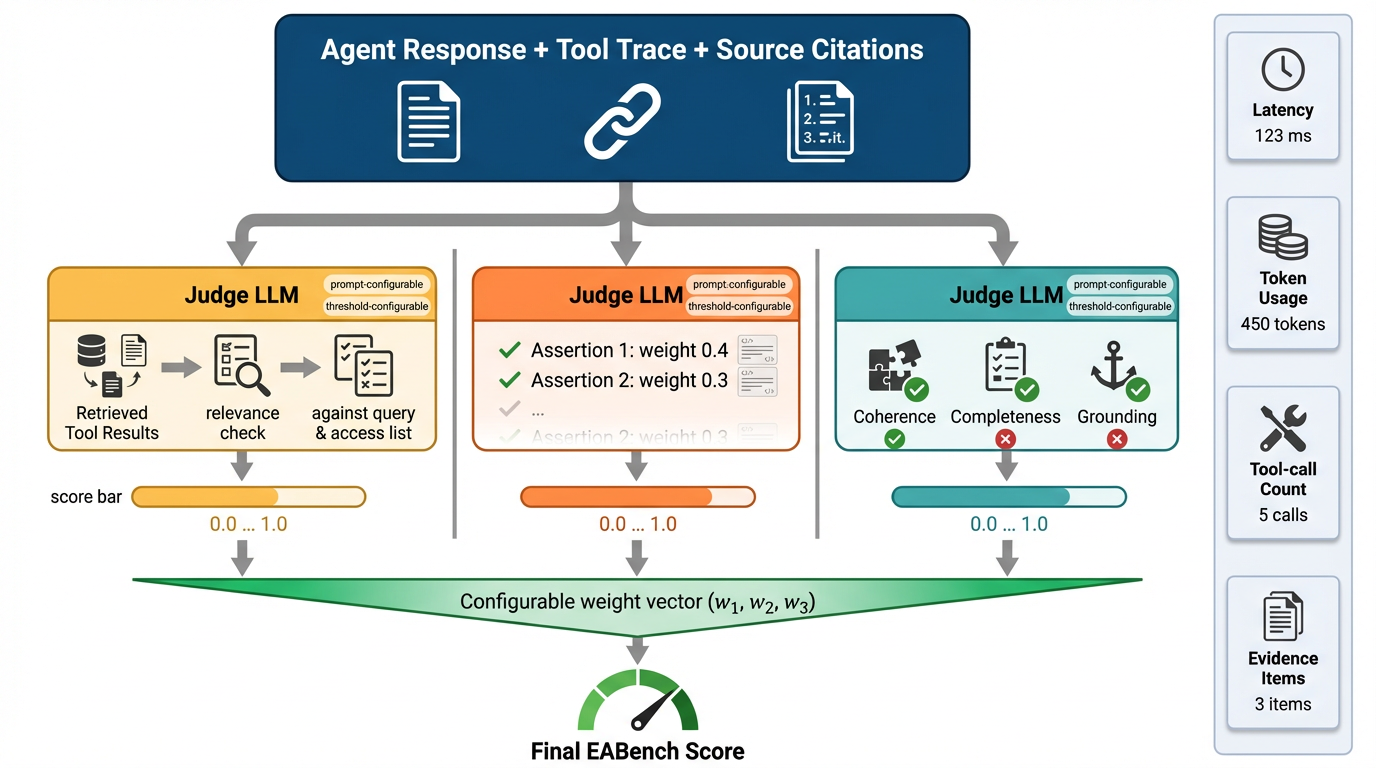
\includegraphics[width=0.9\textwidth]{figures/LLM-as-a-judge-eabench.png}
\caption{EABench multi-dimensional evaluation harness. Two independently configurable LLM-judge tracks score tool-search relevance and response-citation quality; their equal-weight average forms the combined citation score. The assertion score is computed by a third judge call. All three judge scores are reported alongside deterministic diagnostics for operational profiling.}
\label{fig:eval_harness}
\end{figure}

\subsubsection{Pass/Fail Criteria}

A case is marked as passed when both of the following conditions hold simultaneously:
\begin{itemize}[leftmargin=*,itemsep=2pt,topsep=4pt]
  \item \textbf{Assertion score $\geq 0.75$.} At least 75\% of the natural-language assertions are satisfied. This threshold reflects enterprise contexts in which a response missing more than one in four factual requirements is operationally unacceptable.
  \item \textbf{Response-citation quality $\geq 0.7$.} The final answer must include a sufficiently grounded references section. This gate ensures that a plausible-sounding response is still marked as failed if it cites hallucinated artifacts.
\end{itemize}
This dual criterion encodes an important design principle: correctness and grounding are jointly necessary for enterprise-agent success. An agent that satisfies all assertions but fabricates its citations fails the grounding gate; an agent with a well-formed references section that misses key facts fails the correctness gate.

\textcolor{blue}{We do not currently report a human-annotator validation study of assertion grounding, satisfiability, and inter-rater agreement; the assertion-generation pipeline is instead validated indirectly through judge--judge agreement checks and through a post-hoc keyword-based audit of query-type coverage (Section~\ref{sec:experiments}). We treat a full human-annotation study as an open validation task (Section~\ref{sec:threats}).}

\subsubsection{Side-by-Side Comparison and Diagnostics}

For comparative studies, EABench can evaluate two agent configurations on the same case and ask a judge model to declare a winner. These pairwise judgments support win-rate analyses and Bradley--Terry modeling, while the underlying per-case metric vectors support paired tests such as the Wilcoxon signed-rank test. Because the result structure stores the full response, tool trace, assertion outcomes, and citation logs, comparative findings are accompanied by diagnostics that explain why one agent won rather than only whether it won.

\subsubsection{User-Level Experience Simulation}

Evaluation is always grounded in a requesting user context. Before each case is run, the search engine is bound to \texttt{case.user\_id}, and access-control rules are enforced consistently across search results, citation verification, and debugging views. This design allows the same tenant to support engineer, manager, and contractor personas without maintaining separate corpora, and it turns access control into a benchmarked capability rather than an external precondition.
\subsection{Interactive Debugging and Chat Interface}
\label{sec:method_interactive}

\subsubsection{Live Chat Interface}

\textcolor{blue}{Batch evaluation is necessary for aggregate comparison, but it is insufficient for rapid iteration on agent design. EABench therefore ships an interactive Streamlit application (Figure~\ref{fig:debug_interface}) in which the same runtime used for evaluation can be exercised through a live chat interface. A researcher selects an agent configuration, a tenant dataset, and a user persona from the sidebar, then issues free-form queries to inspect the agent's behavior under that persona's access scope. The main panel displays the agent's structured response with inline citation markers and a references section listing source artifacts with metadata (type, author, date, entity ID). This mode is especially valuable during prompt engineering and tool-ablation studies, because it shortens the loop between a configuration change and a concrete behavioral observation.}

\subsubsection{Debugging Facilities}

\textcolor{blue}{The interactive layer exposes the pieces of evidence that matter for debugging enterprise agents. The sidebar navigation provides four views: \emph{Chat} for live query exploration, \emph{Evaluation} for batch result inspection, \emph{Side-by-Side Comparison} for contrasting agent configurations on the same query, and \emph{Data Generator} for creating new tenant datasets. In the Chat view, the agent's response includes inline citation markers that link to a References section with full artifact metadata---type, author, date, and entity ID---enabling a researcher to verify each cited source against the tenant corpus. The Login panel displays the active user's role and ID, making access-scope constraints transparent. These views make it possible to distinguish several common failure modes: the agent may choose the wrong tool, retrieve weak evidence, lose track of a multi-hop chain, or cite the right artifact incorrectly. Because these signals are surfaced directly, EABench supports debugging by diagnosis rather than by prompt trial-and-error alone.}

\begin{table}[t]
\centering
\caption{\textcolor{blue}{Debugging surfaces exposed by the interactive workflow.}}
\label{tab:debug_surfaces}
\small
{\color{blue}
\begin{tabular}{p{0.28\linewidth}p{0.60\linewidth}}
\toprule
\textbf{Surface} & \textbf{What it reveals} \\
\midrule
Agent \& tenant selectors & Switch agent configuration and corpus without restarting \\
User persona login        & Role, user ID, and access scope active for the current session \\
Inline citations          & Numbered markers in the response linking to specific source artifacts \\
References panel          & Full metadata (type, author, date, entity ID) for each cited artifact \\
Side-by-side comparison   & Contrast two agent configurations on the same query and persona \\
Batch evaluation view     & Aggregate metrics and per-case drill-down for completed eval runs \\
\bottomrule
\end{tabular}
}
\end{table}

\begin{figure}[t]
\centering
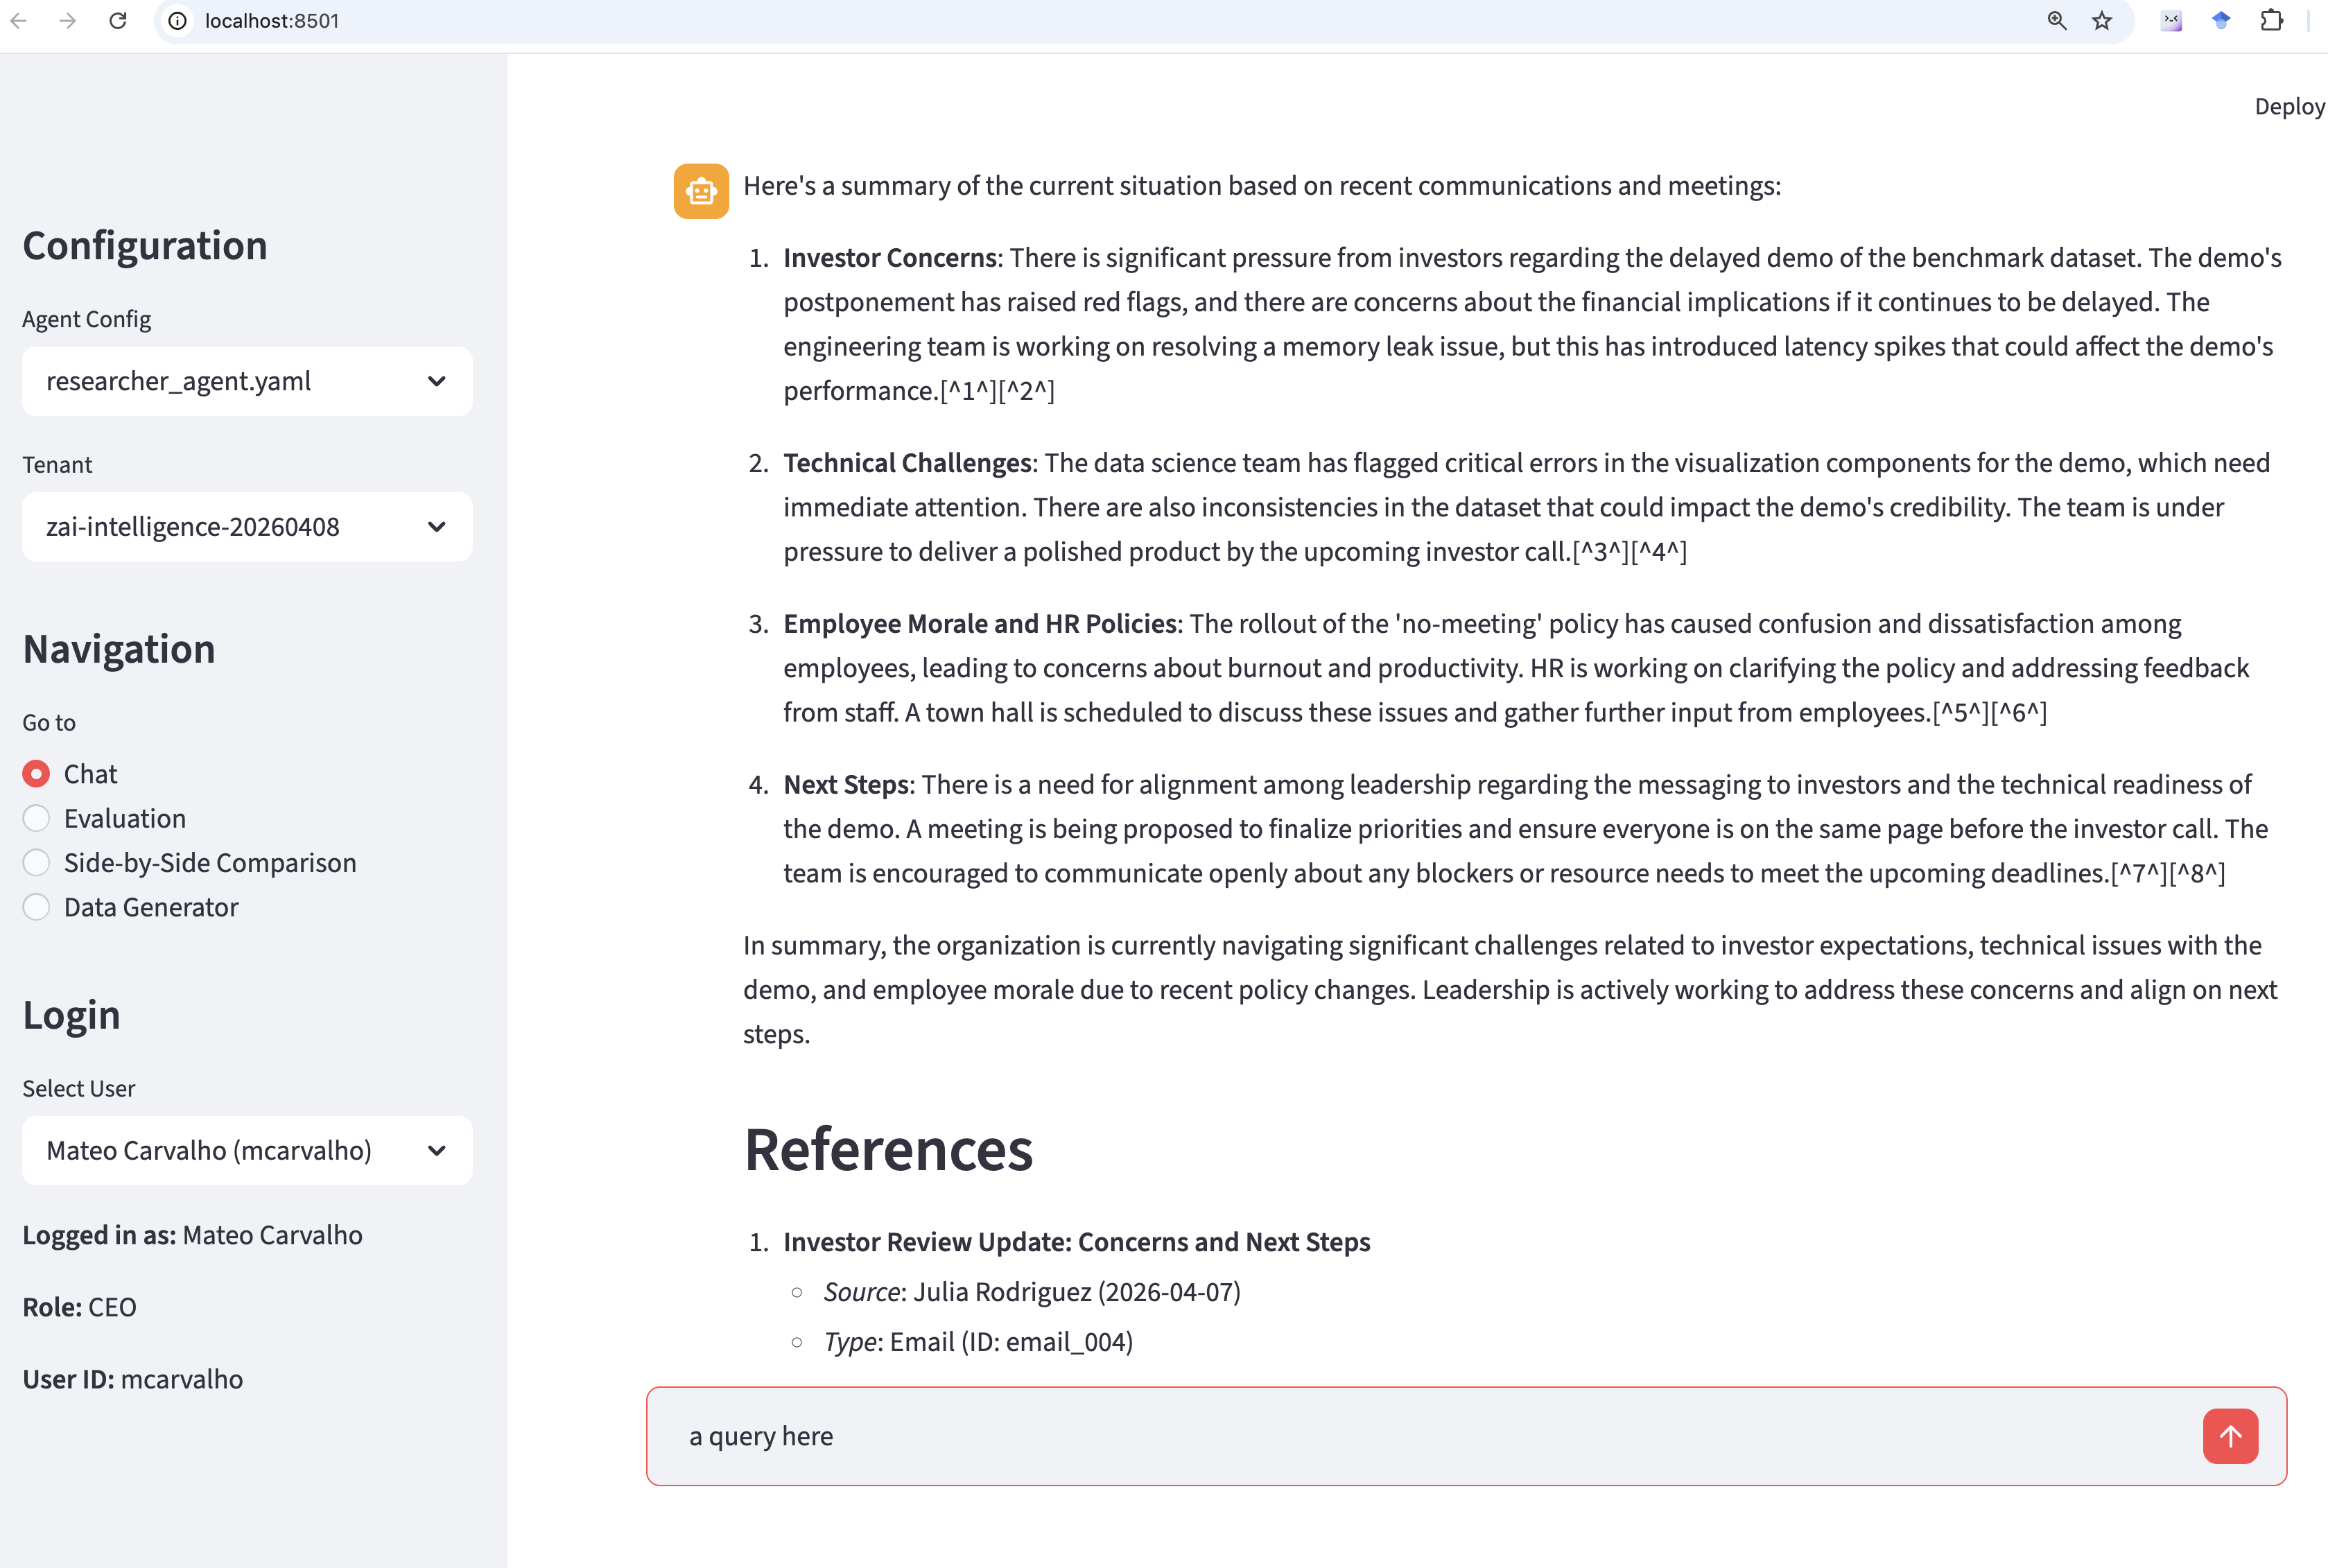
\includegraphics[width=\linewidth]{figures/eabench_screenshot.png}
\caption{\textcolor{blue}{EABench interactive chat interface. The left sidebar provides configuration controls (agent strategy, tenant, and user persona); the main panel displays the agent's structured response with inline citation markers and a references section listing source artifacts with metadata. A query input box at the bottom enables iterative exploration under the selected persona.}}
\label{fig:debug_interface}
\end{figure}

\subsubsection{User Experience Testing}

\textcolor{blue}{The interactive workflow is also useful for evaluating enterprise usability beyond aggregate benchmark scores. Researchers can replay the same case under multiple personas, inspect which artifacts become visible or hidden, and compare how different runtime configurations explain uncertainty to the user. In this sense, the interactive interface serves as a bridge between formal benchmarking and deployment-oriented validation: it preserves reproducibility while surfacing the qualitative details that determine whether an enterprise agent is trustworthy in practice.}


% ══════════════════════════════════════════════════════════════════════
% 4  BENCHMARK SCENARIOS AND INSTANTIATIONS
% ══════════════════════════════════════════════════════════════════════

\section{Benchmark Scenarios and Instantiations}
\label{sec:scenarios}

\textcolor{blue}{To demonstrate how EABench instantiates distinct enterprise workloads without changing the underlying codebase, we define three scenario families that vary organizational structure, confidentiality boundaries, and temporal reasoning demands. The purpose of these scenarios is not merely to populate different datasets; each scenario is designed to stress a different slice of agent capability, including access-aware retrieval, multi-hop reasoning across modalities, and long-form synthesis over multi-day windows. Table~\ref{tab:scenario_map} summarizes the intended stressors.}

\begin{table}[h]
\centering
\caption{\textcolor{blue}{Scenario families used to instantiate EABench and the benchmark capabilities they emphasize.}}
\label{tab:scenario_map}
\small
{\color{blue}
\begin{tabular}{p{0.12\linewidth}p{0.17\linewidth}p{0.23\linewidth}p{0.38\linewidth}}
\toprule
\textbf{Scenario} & \textbf{Primary stressor} & \textbf{Dominant artifacts} & \textbf{Representative evaluation focus} \\
\midrule
Education & Policy evolution across administrative silos & Committee emails, meeting transcripts, planning documents, service-status updates & Timeline reconstruction for curriculum changes, attribution of administrative decisions, and deep-dive reports spanning outages and policy revisions \\
Law firm & Strict confidentiality and role-dependent visibility & Client briefs, internal legal memoranda, partner chats, case meetings & Access-control compliance, privilege-sensitive retrieval, and citation-grounded answers under consultant and attorney personas \\
Software company & Cross-modal incident response and product execution & Incident reports, engineering chats, sprint meetings, launch documents, customer escalation emails & Multi-hop tracing from symptom to root cause, tool-heavy search trajectories, and report generation over short operational windows \\
\bottomrule
\end{tabular}
}
\end{table}

\subsection{Education: University Administrators and Faculty}
\textcolor{blue}{The education scenario models a university-like environment in which decisions emerge through committee processes rather than single-owner workflows. This structure produces queries that require the agent to connect policy drafts, meeting discussions, and follow-up emails over multi-week windows. It is therefore particularly useful for evaluating deep-dive report generation and temporally grounded retrieval, because the correct answer often depends on reconstructing how a proposal evolved across multiple administrative groups rather than locating a single decisive artifact.}

\subsection{Law Firm: Consultants and Attorneys}
\textcolor{blue}{The law-firm scenario emphasizes confidentiality and sharply differentiated access rights. Here the central question is not only whether the agent can retrieve relevant material, but whether it can do so while respecting the requesting user's role. This scenario is especially effective for evaluating user-level experience simulation: the same natural-language request may be answerable for a partner, partially answerable for a staff attorney, and intentionally blocked for a consultant. As a result, the scenario exercises both the retrieval stack and the policy layer that sits on top of it.}

\subsection{Software Company: SDEs and Managers}
\textcolor{blue}{The software-company scenario concentrates dense cross-references into short operational bursts such as outages, launch reviews, and rollback decisions. It is the most tool-intensive scenario because answers frequently require the agent to combine people search, chat retrieval, meeting lookup, and file inspection inside the same trajectory. This makes it a strong stress test for the difference between ReAct and plan-and-execute agents: the former can react quickly to local evidence, while the latter benefits when a multi-step dependency chain must be planned before execution.}

% ══════════════════════════════════════════════════════════════════════
% BENCHMARK DATASET STATISTICS
% Input this file after \section{Benchmark Scenarios and Instantiations}
% ══════════════════════════════════════════════════════════════════════

\subsection{Dataset Statistics}
\label{sec:dataset-stats}

We instantiated EABench across three concrete tenant organizations spanning distinct enterprise domains: a boutique law firm (\emph{Bertrand \& Co.}, 41 users), a mid-size research university (\emph{University of Cambford}, 62 users), and a fast-growing AI startup (\emph{ZAI Intelligence}, 165 users). Each tenant was generated independently by the same GPT-4o-based pipeline described in Section~\ref{sec:method_generation}, parameterized with a domain-specific company description, a set of key narrative events, and an organizational size. The staged generator ensures that artifacts within a single simulated day are mutually coherent---an email thread's content is consistent with the meeting that prompted it---while still allowing realistic variation across days.

Table~\ref{tab:dataset_summary} summarizes the resulting artifact counts and evaluation-case distribution. For each tenant, three evaluation query generators---targeted artifact search, multi-hop reasoning, and comprehensive report---produce structured test cases in a separate pass that examines the completed corpus and constructs questions, gold assertions, and entity lists against it.

\begin{table*}[t]
\centering
\caption{Artifact composition and evaluation case counts for the three EABench tenants.
For chats and group chats, the count reflects distinct conversation threads rather than individual messages.
Evaluation cases span targeted artifact search, multi-hop reasoning, and comprehensive report query types (see Section~\ref{sec:eval-metrics}).}
\label{tab:dataset_summary}
\small
\resizebox{\textwidth}{!}{%
\begin{tabular}{lcccccccccc}
\toprule
\textbf{Tenant} & \textbf{Domain} & \textbf{Users} & \textbf{Emails} & \textbf{DMs} & \textbf{Group} & \textbf{Meetings} & \textbf{Files} & \multicolumn{3}{c}{\textbf{Eval Cases}} \\
\cmidrule(lr){9-11}
 & & & & & \textbf{Chats} & & & \textbf{Tgt.\ Search} & \textbf{Multi-Hop} & \textbf{Compreh.} \\
\midrule
Bertrand \& Co.     & Legal       & 41  & 132 & 56  & 118 & 69  & 70  & 80 & 43 & 39 \\
Univ.\ of Cambford  & Education   & 62  & 120 & 41  & 118 & 70  & 70  & 80 & 44 & 38 \\
ZAI Intelligence    & AI / SW     & 165 & 298 & 140 & 301 & 164 & 164 & 79 & 82 & 40 \\
\midrule
\textbf{Total}      &             & 268 & 550 & 237 & 537 & 303 & 304 & 239 & 169 & 117 \\
\bottomrule
\end{tabular}}
\end{table*}

\noindent The three tenants vary substantially in scale: ZAI Intelligence is roughly four times larger than Bertrand \& Co.\ across every artifact category, and its eval-case count (201) is proportionally expanded to maintain per-tenant statistical power. This heterogeneity is intentional---EABench is designed to stress-test agents under differing information densities rather than to standardize them away.

The query-type distribution follows the pipeline's target split of approximately 40/40/20 (targeted artifact search / multi-hop reasoning / comprehensive report). The actual ratios deviate slightly because each generator produces variable-sized batches. Targeted artifact search queries each reference exactly one gold entity, multi-hop reasoning queries reference 2--5 entities from different modalities, and comprehensive report queries reference 3--15 entities spanning multiple artifact types and dates.

\begin{table}[h]
\centering
\caption{Ground-truth evaluation complexity by query type and tenant.
``Assertions'' are gold-standard factual statements the agent's response must satisfy;
``Entities'' are the ground-truth artifacts (emails, chats, meetings, files) required to answer the query.}
\label{tab:ground_truth}
\small
\begin{tabular}{llcccccc}
\toprule
& & \multicolumn{3}{c}{\textbf{Assertions per Case}} & \multicolumn{3}{c}{\textbf{Entities per Case}} \\
\cmidrule(lr){3-5} \cmidrule(lr){6-8}
\textbf{Tenant} & \textbf{Query Type} & \textbf{Mean} & \textbf{Med.} & \textbf{Range} & \textbf{Mean} & \textbf{Med.} & \textbf{Range} \\
\midrule
\multirow{3}{*}{Bertrand}
  & Targeted Artifact Search  & 2.4 & 2 & 2--4  & 1.0 & 1 & 1--1  \\
  & Multi-Hop Reasoning        & 2.3 & 2 & 2--3  & 2.7 & 2 & 2--5  \\
  & Comprehensive Report       & 3.2 & 3 & 3--4  & 5.3 & 5 & 4--10 \\
\midrule
\multirow{3}{*}{Cambford}
  & Targeted Artifact Search  & 2.6 & 3 & 2--3  & 1.0 & 1 & 0--1  \\
  & Multi-Hop Reasoning        & 2.8 & 3 & 2--4  & 3.1 & 3 & 2--4  \\
  & Comprehensive Report       & 3.2 & 3 & 3--4  & 5.9 & 5 & 3--15 \\
\midrule
\multirow{3}{*}{ZAI}
  & Targeted Artifact Search  & 2.2 & 2 & 2--3  & 1.0 & 1 & 1--1  \\
  & Multi-Hop Reasoning        & 2.3 & 2 & 2--5  & 2.4 & 2 & 2--5  \\
  & Comprehensive Report       & 3.2 & 3 & 3--4  & 6.0 & 5 & 3--11 \\
\bottomrule
\end{tabular}
\end{table}

\noindent Table~\ref{tab:ground_truth} reveals a clear complexity gradient across query types. Targeted artifact search queries average 2.2--2.6 assertions grounded in a single entity, making them the simplest evaluation targets. Multi-hop reasoning queries maintain a similar assertion count but require cross-referencing 2--5 entities from different communication modalities. Comprehensive report queries demand the most complex synthesis: 3--4 assertions each backed by 3--15 source entities spanning emails, chats, meetings, and files. This structured complexity scaling ensures that the evaluation set probes agent capabilities at multiple difficulty levels.

\subsection{Communication Network Properties}
\label{sec:network-stats}

To characterize inter-personal communication structure, we extract a directed multigraph for each tenant in which nodes are users and edges represent recorded communicative acts across five channel types: email (\emph{from}$\to$\emph{to}), email CC (\emph{from}$\to$\emph{cc}), direct-message chat (\emph{sender}$\to$\emph{recipient}), group chat (\emph{sender}$\to$all participants), and meeting (pairwise edges among all attendees plus \emph{organizer}$\to$\emph{attendee} edges). Table~\ref{tab:network_metrics} reports standard graph-theoretic properties for each tenant's aggregate communication network.

\begin{table}[h]
\centering
\caption{Communication network topology for each tenant.
Density $= |E| / (|V|(|V|-1))$ for a directed graph.
Reciprocity is the fraction of directed edges that have a reverse edge.
Transitivity is the global clustering coefficient.
$\gamma$ is the exponent of the power-law fit $P(k) \sim k^{-\gamma}$ to the in-degree complementary cumulative distribution (CCDF), with $R^2$ the goodness-of-fit.}
\label{tab:network_metrics}
\small
\begin{tabular}{lccccccccc}
\toprule
\textbf{Tenant} & \textbf{$|V|$} & \textbf{$|E|$} & \textbf{Density} & \textbf{Diam.} & \textbf{Avg.\ Path} & \textbf{Recip.} & \textbf{Trans.} & \textbf{$\gamma$} & \textbf{$R^2$} \\
\midrule
Bertrand       & 41  & 322   & 0.196 & 3 & 1.71 & 0.286 & 0.486 & 0.36 & 0.29 \\
Cambford       & 62  & 519   & 0.137 & 4 & 1.89 & 0.343 & 0.448 & 0.68 & 0.42 \\
ZAI            & 165 & 1{,}956 & 0.072 & 4 & 2.10 & 0.314 & 0.367 & 0.66 & 0.59 \\
\bottomrule
\end{tabular}
\end{table}

\begin{figure}[h]
\centering
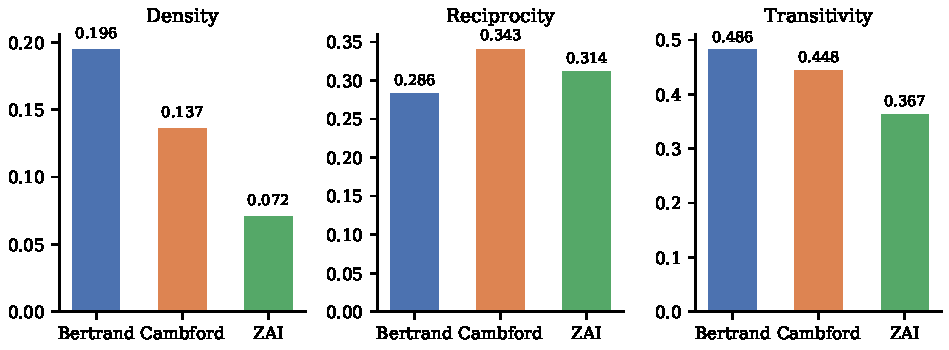
\includegraphics[width=0.85\linewidth]{figures/network_comparison.pdf}
\caption{Key communication-network metrics across the three EABench tenants. Density, reciprocity, and transitivity decrease with organizational scale, reflecting the transition from tight-knit professional-services firms to large engineering organizations with departmental silos.}
\label{fig:network_comparison}
\end{figure}

\noindent These metrics reflect realistic organizational archetypes. Bertrand \& Co., the smallest organization, is the densest (0.196) and has the smallest diameter (3), consistent with a tight-knit professional-services firm where most colleagues interact directly. ZAI Intelligence, the largest, exhibits a sparse, long-tail structure (density~0.072, 1{,}956 edges among 165~nodes) typical of rapidly growing technology companies with departmental silos. The University of Cambford occupies an intermediate position with the highest reciprocity (0.343), reflecting the collaborative back-and-forth characteristic of academic committee work. Transitivity is highest for Bertrand (0.486), where shared client matters create strong triadic closure, and lowest for ZAI (0.367), where cross-functional interaction is sparser.

The in-degree distributions follow a heavy-tailed pattern. We fit a power law $P(k) \sim k^{-\gamma}$ to the complementary cumulative distribution of in-degrees and compare the empirical graph against a synthetic Barab\'{a}si--Albert (BA) preferential-attachment graph of the same size. The low $\gamma$ values (0.36--0.68) confirm that all three networks exhibit right-skewed degree distributions rather than Poisson-like regularity. The $R^2$ values increase with tenant size (0.29 for Bertrand, 0.59 for ZAI), indicating that the power-law fit improves as the number of nodes permits a wider degree range. In each case, the maximum in-degree substantially exceeds the BA model's prediction (e.g., 99 vs.\ 72 for ZAI, 43 vs.\ 34 for Cambford), indicating that the generated organizations produce realistic ``hub'' individuals---such as executives, team leads, or central administrative staff---whose communication connectivity is disproportionately high.

Per-channel decomposition reveals further structural realism. Email communication has reciprocity between 0.48 and 0.73 across tenants, reflecting the natural tendency for emails to receive replies. Chat messages are entirely non-reciprocal at the edge level (0.0), since each message is a directed act from sender to recipient with no guaranteed return in the same thread. Meeting edges, constructed from attendee co-presence, are fully reciprocal by construction (1.0). This channel-level heterogeneity is important for evaluation: an agent that reasons about ``who communicated with whom'' must integrate evidence from channels with qualitatively different relational semantics.

\subsection{Temporal Communication Patterns}
\label{sec:temporal-stats}

Realistic enterprise datasets exhibit bursty temporal structure: communication tends to cluster around deadlines, incidents, or scheduled events rather than arriving as a uniform Poisson process. We quantify this using the burstiness parameter $B = (\sigma_\tau - \mu_\tau) / (\sigma_\tau + \mu_\tau)$, where $\mu_\tau$ and $\sigma_\tau$ are the mean and standard deviation of the inter-event time (IET) sequence for a given communication channel~\cite{goh2008burstiness}. Values of $B$ near zero indicate exponential (Poisson) inter-arrival times, while $B > 0$ indicates bursty clustering. We additionally report the memory coefficient $M$~\cite{goh2008burstiness}, which measures the correlation between consecutive IETs: $M > 0$ indicates that long gaps tend to follow long gaps (temporal clustering at multiple scales), while $M \approx 0$ indicates uncorrelated consecutive intervals.

\begin{table}[h]
\centering
\caption{Inter-event time (IET) statistics per communication channel and tenant.
Burstiness $B > 0$ indicates clustered arrivals; $B \approx 0$ indicates near-Poisson behavior.
Memory coefficient $M$ measures serial correlation between consecutive IETs.
$\alpha$ is the power-law exponent fitted to the IET distribution. Meeting channels are omitted for brevity (their $|B| < 0.01$ in all tenants except ZAI, where $B = 0.23$ with $M = 0.19$).}
\label{tab:iet_summary}
\small
\begin{tabular}{llccccc}
\toprule
\textbf{Tenant} & \textbf{Channel} & \textbf{Events} & \textbf{$B$} & \textbf{$M$} & \textbf{$\alpha$} & \textbf{Med.\ IET (s)} \\
\midrule
\multirow{3}{*}{Bertrand}
  & Email      & 132   & $-$0.051 & $-$0.054 & 2.00 & 81{,}450 \\
  & Chat (1:1) & 1{,}022 & $+$0.617 & $-$0.055 & 0.33 & 72       \\
  & Group Chat & 2{,}291 & $+$0.560 & $-$0.078 & 0.36 & 120      \\
\midrule
\multirow{3}{*}{Cambford}
  & Email      & 120   & $+$0.065 & $-$0.045 & 1.49 & 85{,}500 \\
  & Chat (1:1) & 732   & $+$0.640 & $-$0.048 & 0.35 & 90       \\
  & Group Chat & 2{,}075 & $+$0.575 & $-$0.072 & 0.34 & 110      \\
\midrule
\multirow{3}{*}{ZAI}
  & Email      & 298   & $+$0.168 & $+$0.395 & 1.28 & 82{,}800 \\
  & Chat (1:1) & 2{,}581 & $+$0.658 & $-$0.042 & 0.33 & 77       \\
  & Group Chat & 6{,}033 & $+$0.614 & $-$0.055 & 0.31 & 150      \\
\bottomrule
\end{tabular}
\end{table}

\noindent The results validate that EABench's generation pipeline reproduces two hallmarks of real organizational communication. First, email arrivals are near-Poisson ($B \approx 0$) across all three tenants, with high $\alpha$ values (1.28--2.00) indicating that inter-arrival times decay rapidly---consistent with the scheduled nature of formal correspondence. Second, chat and group-chat streams are highly bursty ($B \in [0.56, 0.66]$) with low power-law exponents ($\alpha \in [0.31, 0.36]$), confirming heavy-tailed inter-event time distributions where short bursts of rapid-fire messages are separated by long silences. This pattern matches empirical measurements of instant-messaging platforms in organizational settings~\cite{goh2008burstiness}.

The memory coefficients are near zero for most channel--tenant pairs ($M \in [-0.08, 0.0]$), indicating that the IET process is approximately memoryless at the single-channel level---as expected when daily narrative generation does not explicitly model autoregressive temporal dependence within a channel. The notable exception is ZAI's email channel ($M = +0.40$), where the organizational scale produces enough correlated event clusters (e.g., multi-day incident threads, product-launch email bursts) to induce measurable serial dependence.

This temporal structure directly impacts retrieval difficulty: an agent must reason about \emph{when} information was generated, not only \emph{what} it contains, because a correct multi-hop answer often depends on reconstructing an event sequence from artifacts whose timestamps are concentrated in bursty clusters rather than distributed uniformly.


% ══════════════════════════════════════════════════════════════════════
% 5  EXPERIMENTS
% ══════════════════════════════════════════════════════════════════════

\section{Experiments}
\label{sec:experiments}

EABench is designed to support controlled experimentation rather than a single fixed leaderboard. We organize this section around the experimental protocol: a description of the setup and metric definitions, followed by empirical results across three agent configurations and three tenant scenarios, ablation studies isolating the contribution of architectural and prompt-engineering choices, and an analysis of the cost-effectiveness frontier. Table~\ref{tab:exp_matrix} summarizes the core experimental design.

\begin{table}[h]
\centering
\caption{Core experimental protocol supported by EABench.}
\label{tab:exp_matrix}
\small
\begin{tabular}{p{0.17\linewidth}p{0.26\linewidth}p{0.18\linewidth}p{0.28\linewidth}}
\toprule
\textbf{Axis} & \textbf{Controlled variables} & \textbf{Primary outputs} & \textbf{Purpose} \\
\midrule
Cross-model evaluation & Tenant generator, runtime model, judge model, flow strategy & Pass rate, assertion score, citation score, win rate & Detect self-preference bias; verify ranking stability across generator--judge combinations \\
Ablation studies & Architecture (ReAct vs.\ plan-and-execute), prompt verbosity, execution temperature, tool configuration & Metric deltas per agent--tenant cell & Attribute performance to specific platform components \\
Scenario analysis & Industry template, company size, event density, persona mix & Per-scenario score distribution, failure taxonomy, latency diagnostics & Determine which scenario characteristics most affect retrieval, reasoning, and citation \\
\bottomrule
\end{tabular}
\end{table}

\subsection{Experimental Setup}
\label{sec:exp-setup}

We instantiate the three scenario families from Section~\ref{sec:scenarios} as concrete tenants (Bertrand \& Co., University of Cambford, and ZAI Intelligence) and evaluate three agent configurations that span a spectrum from minimal reactive reasoning to deliberative planning. All agents share the same embedding model (\texttt{text-embedding-ada-002}) and use GPT-4o-family models via Azure OpenAI: the two ReAct agents use GPT-4o while the Researcher agent uses GPT-4o-mini for both planning and execution. The automated judge is GPT-4o at temperature~0.0, evaluating each case via four separate LLM calls that measure assertion satisfaction, tool-search relevance, and response-citation quality. Each agent is evaluated on all 525 cases (162 per small tenant, 201 for ZAI) covering three query types: search, multi-hop, and report. We record both judge-based quality metrics and deterministic operational diagnostics---latency, token usage, tool-call count, and retrieval volume---to distinguish capability failures from operational inefficiency.

% ══════════════════════════════════════════════════════════════════════
% EMPIRICAL RESULTS — AGENT × TENANT EVALUATION
% Input this file inside \section{Experiments}, after \subsection{Experimental Setup}
% ══════════════════════════════════════════════════════════════════════

\subsubsection{Agent Configurations}
\label{sec:agent-configs}

We evaluate three agent configurations whose designs span a spectrum from minimal reactive reasoning to deliberative multi-step planning. All three share the same embedding model (\texttt{text-embedding-ada-002}) and use GPT-4o-family models via Azure OpenAI: the two ReAct agents use GPT-4o while the Researcher agent uses GPT-4o-mini. This design varies architecture, prompt engineering, and model size simultaneously, reflecting the realistic design space in which practitioners choose agent configurations.

\begin{table}[h]
\centering
\caption{Configuration summary for the three evaluated agents.
``Planning model'' refers to the LLM used for the optional pre-execution planning step.
Prompt size is the approximate system-prompt token count. Avg.\ tool calls and latency are empirical means across all evaluation cases.}
\label{tab:agent_configs}
\small
\begin{tabular}{p{0.12\linewidth}p{0.12\linewidth}p{0.12\linewidth}p{0.06\linewidth}p{0.10\linewidth}p{0.10\linewidth}p{0.10\linewidth}p{0.10\linewidth}}
\toprule
\textbf{Agent} & \textbf{Architecture} & \textbf{Model} & \textbf{$T$} & \textbf{Planning Model} & \textbf{Prompt Size} & \textbf{Avg.\ Tools} & \textbf{Avg.\ Lat.\ (s)} \\
\midrule
\textsc{ReAct-v1}   & Single-pass ReAct & GPT-4o      & 0.7 & ---               & $\sim$3k tok   & 1.70 & 17.6 \\
\textsc{ReAct-v2}   & Single-pass ReAct & GPT-4o      & 0.5 & ---               & $\sim$1.5k tok & 1.70 & 18.2 \\
\textsc{Researcher}  & Plan\,+\,Execute  & GPT-4o-mini & 0.0 & GPT-4o-mini ($T{=}0$) & $\sim$3k tok   & 4.85 & 65.2 \\
\bottomrule
\end{tabular}
\end{table}

\textsc{ReAct-v1} implements a standard ReAct loop~\cite{yao2022react} with a verbose system prompt ($\sim$3{,}000 tokens) containing eight fully worked \textsc{Thought}$\to$\textsc{Tool} examples. These examples concretely demonstrate several critical behavioral patterns: dual-term person lookup (searching simultaneously by display name and by user~ID), pronoun-to-ID resolution before issuing any content search, multi-query decomposition for relationship-based questions (``emails between A and B''), and detailed citation formatting with per-fact inline superscripts and a mandatory \texttt{\#\# References} section listing artifact IDs. Its execution temperature of 0.7 permits exploratory variation in search-query phrasing.

\textsc{ReAct-v2} shares the same single-pass ReAct loop but condenses the system prompt to $\sim$1{,}500 tokens across five terse bullet-style examples. The instructions cover the same topics---people resolution, citation formatting, pronoun disambiguation---but omit the extended worked demonstrations, replacing them with one-line directives. Its execution temperature is lowered to 0.5.

\textsc{Researcher} introduces a dedicated planning stage: GPT-4o-mini (at temperature~0.0) first generates a structured, step-by-step research plan before any tool call is issued. The planning prompt explicitly requires four capabilities: (i)~\emph{multi-hop reasoning}---decomposing complex questions into dependency chains; (ii)~\emph{correlated search}---cross-referencing across emails, chats, meetings, and files; (iii)~\emph{mandatory ID resolution}---resolving names to user IDs via \texttt{search\_people} before any content search; and (iv)~\emph{step-by-step ordering}---arranging steps so that the output of each feeds the next. The planner is instructed to output only the plan, not to execute it. The same GPT-4o-mini model (at temperature~0.0) then executes the plan step by step using the full tool set, resulting in systematically broader retrieval (61.6 items retrieved per case vs.\ 15--19 for the reactive agents) and substantially higher token consumption ($\sim$92k prompt tokens vs.\ $\sim$18k). Notably, despite using a smaller model than the ReAct agents, the Researcher achieves the highest pass rate, demonstrating that structured planning can compensate for reduced per-call model capacity.

\subsubsection{Evaluation Metrics}
\label{sec:eval-metrics}

Each evaluation case consists of a natural-language query, a requesting user identity, a list of gold-standard factual assertions, and a list of entity references that a correct answer should cite. Three query generators produce cases of increasing complexity:

\begin{enumerate}[leftmargin=*,nosep]
\item \textbf{Search queries} target the retrieval of specific items with filtering constraints (e.g., ``Find emails sent by Lisa about fund Beta in the last two weeks'').
\item \textbf{Multi-hop queries} require chaining evidence across artifact types and resolving entity relationships (e.g., ``Who attended the meeting where the Q3 budget was discussed, and what follow-up action did they take by email?'').
\item \textbf{Report queries} request synthesis or summary generation over multi-day windows (e.g., ``Provide a timeline of all decisions related to the server migration from March 1 to March 15'').
\end{enumerate}

\noindent The automated judge (GPT-4o, temperature~0.0) computes four complementary metrics via separate LLM calls:

\paragraph{Assertion score.} Each gold assertion $a_i$ is verified independently against the agent's response. The judge outputs a Boolean \emph{True}/\emph{False} per assertion together with a brief explanation, and the final assertion score for the case is the fraction of assertions satisfied: $\text{Assr.} = |\{a_i : \text{True}\}| / |A|$.

\paragraph{Tool-search relevance.} The judge evaluates three aspects of the agent's tool usage in a single call: (i)~whether the tool calls were \emph{appropriate} for the query, (ii)~whether the retrieved evidence was \emph{relevant} to the question, and (iii)~whether the final response is \emph{grounded} in the retrieved artifacts rather than hallucinated. The result is a scalar relevance score in $[0,1]$. We additionally record the number of items retrieved per case (\emph{tool-search count}).

\paragraph{Response-citation quality.} A separate judge call inspects the response's \texttt{\#\# References} section, checking (i)~whether one exists, (ii)~how many cited artifact IDs are \emph{grounded} (i.e., appear in the tool-call results) versus \emph{hallucinated} (fabricated IDs), and (iii)~whether inline citation markers appear in the response body. The score is in $[0,1]$; we also record the raw grounded-citation count.

\paragraph{Pass rate.} A case is marked \emph{passed} if the assertion score is~1.0 (all assertions satisfied). Pass rate is the fraction of cases that pass.

\noindent For aggregate reporting, we define a composite \emph{citation score} as the mean of tool-search relevance and response-citation quality. This decomposition is important because the two sub-scores measure different failure modes: an agent can retrieve excellent evidence but fail to format citations (high tool-search, low response-citation), or it can produce well-formatted references that point to irrelevant material (low tool-search, high response-citation).

\subsubsection{Main Results}
\label{sec:main-results}

Table~\ref{tab:results_full} reports the decomposed metrics across all nine agent--tenant combinations. Table~\ref{tab:agent_ranking} aggregates results across tenants.

\begin{table}[h]
\centering
\caption{Per-tenant and per-agent evaluation results.
\emph{Pass}: pass rate. \emph{Assr.}: assertion score. \emph{TS-Rel}: tool-search relevance. \emph{TS-$n$}: mean items retrieved. \emph{RC-Rel}: response-citation relevance. \emph{RC-$n$}: mean grounded citations. \emph{Cite}: composite citation score (mean of TS-Rel and RC-Rel). \emph{Lat.}: mean latency in seconds.
Bold marks the best per-tenant value.}
\label{tab:results_full}
\resizebox{\linewidth}{!}{%
\begin{tabular}{llcccccccc}
\toprule
\textbf{Tenant} & \textbf{Agent} & \textbf{Cases} & \textbf{Pass} & \textbf{Assr.} & \textbf{TS-Rel} & \textbf{TS-$n$} & \textbf{RC-Rel} & \textbf{Cite} & \textbf{Lat.\ (s)} \\
\midrule
\multirow{3}{*}{Bertrand}
  & \textsc{ReAct-v1}   & 162 & 0.414              & \textbf{0.736} & \textbf{0.803} & 19.2 & 0.593              & 0.698              & \textbf{18.1} \\
  & \textsc{ReAct-v2}   & 162 & 0.259              & 0.729          & 0.650          & 15.8 & 0.479              & 0.565              & 22.2 \\
  & \textsc{Researcher}  & 162 & \textbf{0.432}     & 0.625          & 0.762          & \textbf{61.1} & \textbf{0.640}     & \textbf{0.701}     & 71.0 \\
\midrule
\multirow{3}{*}{Cambford}
  & \textsc{ReAct-v1}   & 162 & 0.228              & \textbf{0.515} & 0.717          & 18.3 & 0.449              & 0.583              & 17.3 \\
  & \textsc{ReAct-v2}   & 162 & 0.222              & 0.489          & 0.701          & 17.0 & 0.440              & 0.571              & \textbf{15.8} \\
  & \textsc{Researcher}  & 162 & \textbf{0.346}     & 0.543          & \textbf{0.793} & \textbf{61.1} & \textbf{0.684}     & \textbf{0.738}     & 55.3 \\
\midrule
\multirow{3}{*}{ZAI}
  & \textsc{ReAct-v1}   & 201 & 0.269              & \textbf{0.560} & \textbf{0.797} & 17.9 & 0.558              & \textbf{0.677}     & \textbf{19.1} \\
  & \textsc{ReAct-v2}   & 201 & 0.154              & 0.473          & 0.717          & 13.5 & 0.493              & 0.605              & 16.5 \\
  & \textsc{Researcher}  & 201 & \textbf{0.289}     & 0.503          & 0.765          & \textbf{62.5} & \textbf{0.623}     & 0.694              & 69.1 \\
\bottomrule
\end{tabular}
}
\end{table}

\begin{table}[h]
\centering
\caption{Aggregate agent rankings across all three tenants.
Columns follow the same conventions as Table~\ref{tab:results_full}.
\emph{Prompt tok.}: mean input tokens per inference call. \emph{Tool calls}: mean tool invocations per case.}
\label{tab:agent_ranking}

\begin{figure}[h]
\centering
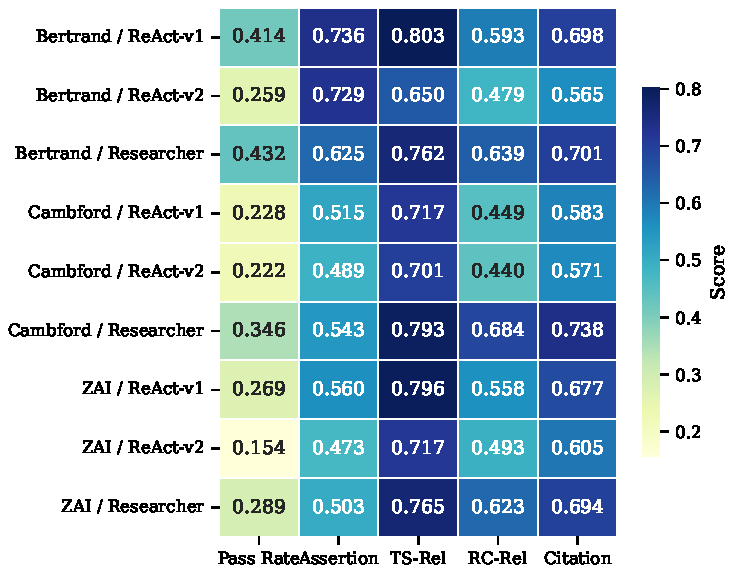
\includegraphics[width=0.9\linewidth]{figures/metrics_heatmap.pdf}
\caption{Evaluation metrics heatmap across all nine agent--tenant combinations. Darker cells indicate higher values. The heatmap provides a compact visual summary of the strengths and weaknesses of each agent configuration across tenants and metric dimensions.}
\label{fig:metrics_heatmap}
\end{figure}

\small
\begin{tabular}{lcccccccccc}
\toprule
\textbf{Agent} & \textbf{Pass} & \textbf{Assr.} & \textbf{TS-Rel} & \textbf{TS-$n$} & \textbf{RC-Rel} & \textbf{RC-$n$} & \textbf{Cite} & \textbf{Lat.\ (s)} & \textbf{Tools} & \textbf{Prompt tok.} \\
\midrule
\textsc{Researcher}  & \textbf{0.355} & 0.557          & 0.773          & \textbf{61.6} & \textbf{0.649} & \textbf{2.81} & \textbf{0.711} & 65.2          & \textbf{4.85} & 92{,}280 \\
\textsc{ReAct-v1}   & 0.323          & \textbf{0.638} & \textbf{0.799} & 18.5          & 0.551          & 1.87          & 0.675          & \textbf{17.6} & 1.70          & 17{,}778 \\
\textsc{ReAct-v2}   & 0.212          & 0.564          & 0.689          & 15.4          & 0.471          & 1.84          & 0.580          & 18.2          & 1.70          & 17{,}203 \\
\bottomrule
\end{tabular}
\end{table}

\begin{figure}[h]
\centering
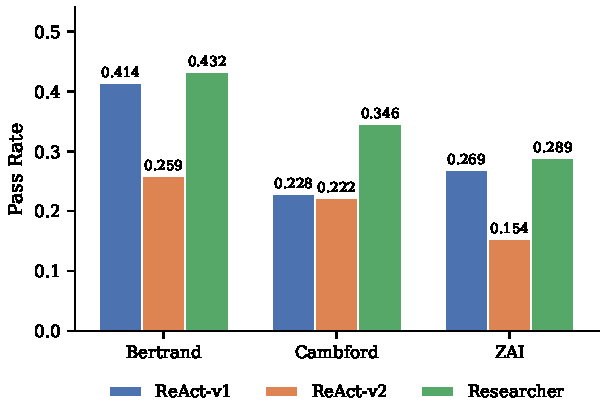
\includegraphics[width=0.9\linewidth]{figures/pass_rate_by_agent_tenant.pdf}
\caption{Pass rate (fraction of cases with all assertions satisfied) by agent configuration and tenant. \textsc{Researcher} leads on Bertrand and Cambford; the gap narrows on ZAI where evidence is temporally concentrated.}
\label{fig:pass_rate}
\end{figure}

\begin{figure}[h]
\centering
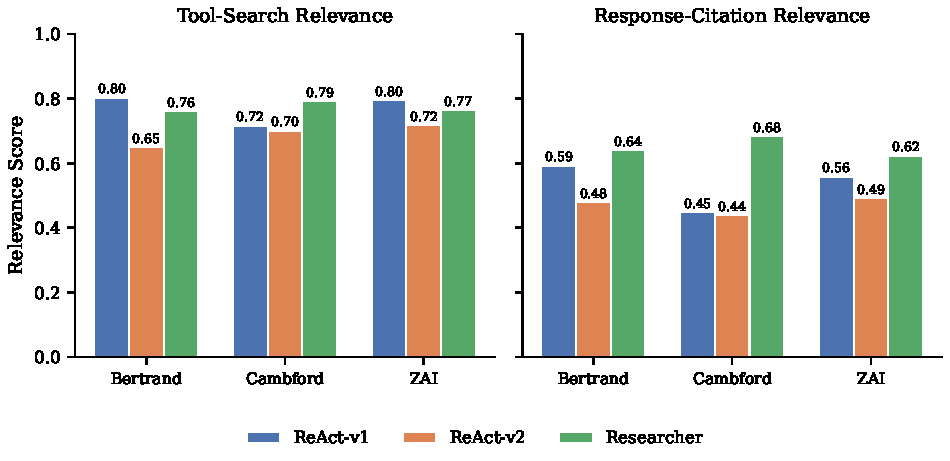
\includegraphics[width=0.9\linewidth]{figures/citation_decomposition.pdf}
\caption{Decomposed citation metrics. \textsc{ReAct-v1} leads on tool-search relevance (left) while \textsc{Researcher} leads on response-citation quality (right), showing that retrieval precision and citation formatting are largely independent failure modes.}
\label{fig:citation_decomp}
\end{figure}

\begin{figure}[h]
\centering
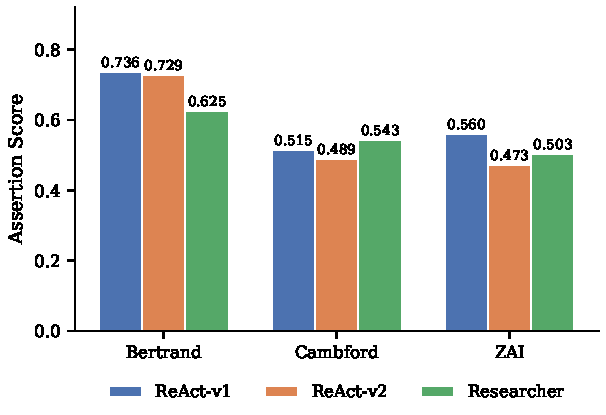
\includegraphics[width=0.9\linewidth]{figures/assertion_score_by_agent_tenant.pdf}
\caption{Mean assertion score (fraction of gold assertions satisfied) by agent and tenant. \textsc{ReAct-v1} leads on factual precision across all three tenants, while \textsc{Researcher}'s broad retrieval strategy sacrifices per-assertion accuracy for coverage.}
\label{fig:assertion_score}
\end{figure}

\noindent \textsc{Researcher} achieves the highest overall pass rate (35.5\%) and citation quality (0.711) but the lowest assertion score (0.557). \textsc{ReAct-v1} ranks second on pass rate (32.3\%) while leading on assertion accuracy (0.638) and tool-search relevance (0.799). \textsc{ReAct-v2} trails on all quality metrics (pass 21.2\%, citation 0.580) despite its structural similarity to v1. The decomposed citation scores reveal that \textsc{Researcher}'s advantage is concentrated in response-citation quality (0.649 vs.\ 0.551 for v1), while \textsc{ReAct-v1} actually leads on tool-search relevance (0.799 vs.\ 0.773). This means that the reactive agent retrieves slightly more relevant evidence per tool call, but the planning agent produces better-structured reference sections because its broader retrieval footprint provides more citable material.

\subsubsection{Effect of Agent Architecture: Plan-and-Execute vs.\ ReAct}
\label{sec:arch-analysis}

The primary architectural difference between \textsc{Researcher} and the two reactive agents is the separation of planning from execution. Before issuing any tool call, \textsc{Researcher} prompts GPT-4o-mini to produce a structured research plan that decomposes the query into a dependency chain, identifies which data modalities to cross-reference, and mandates people-ID resolution before any content search. This design directly explains three empirical patterns.

First, \textsc{Researcher} retrieves 61.6 items per case versus 15--19 for the reactive agents---a factor of $\sim$3.5$\times$. The planning prompt explicitly requires correlated search across emails, chats, meetings, and files, whereas the reactive agents only pursue additional artifact types opportunistically. This broader retrieval footprint is the primary driver of the response-citation advantage: with more retrieved artifacts available, the execution model has more material to cite, raising the grounded-citation count from 1.87 (v1) to 2.81 (\textsc{Researcher}).

\begin{figure}[h]
\centering
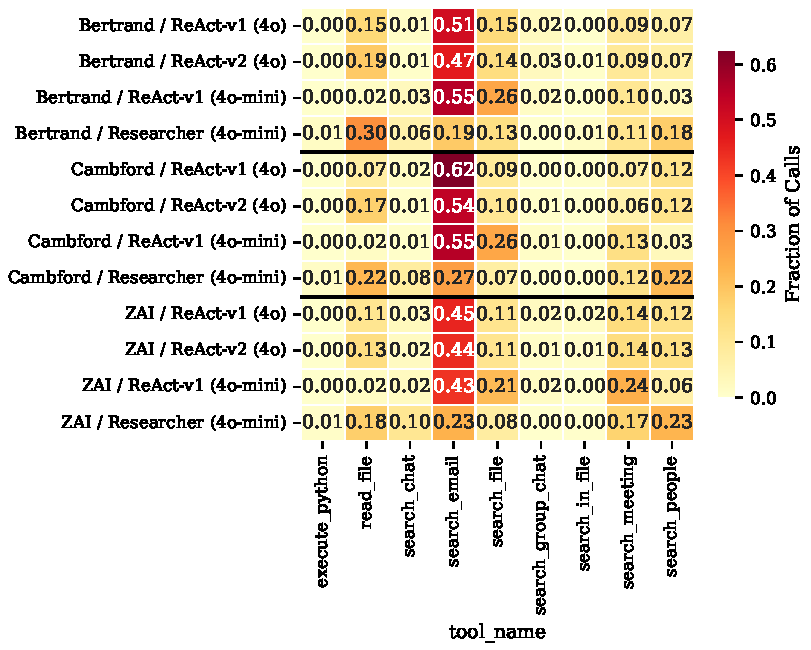
\includegraphics[width=0.9\linewidth]{figures/tool_usage_heatmap.pdf}
\caption{Tool-call distribution by agent and tenant. Rows are grouped by tenant; columns show individual tools. \textsc{Researcher} allocates calls across more tool types in every tenant, while the reactive agents concentrate on \texttt{search\_messages} and \texttt{search\_people}. Cross-tenant variation is visible: ZAI's larger corpus drives higher \texttt{read\_file} usage across all agents.}
\label{fig:tool_usage}
\end{figure}

Second, the planning stage is most beneficial when queries require temporal multi-hop reasoning. On Cambford, where cases frequently require reconstructing policy evolution across weeks of committee emails and subsequent meeting threads, \textsc{Researcher} improves pass rate by 52\% relative to \textsc{ReAct-v1} (0.346 vs.\ 0.228) and achieves the highest citation score in any cell (0.738). On Bertrand, where the smaller, denser organization makes most answers reachable via a single well-formed search, the pass-rate gap shrinks to 4\% (0.432 vs.\ 0.414). On ZAI, where evidence is concentrated in dense operational bursts, \textsc{ReAct-v1} closes to within 2 percentage points of \textsc{Researcher} on pass rate (0.269 vs.\ 0.289) and substantially exceeds it on assertion score (0.560 vs.\ 0.503).

Third, despite leading on pass rate and citation, \textsc{Researcher} lags on assertion score (0.557 vs.\ 0.638 for v1). Two factors contribute: the smaller GPT-4o-mini model has lower per-call reasoning capacity than GPT-4o, and the deterministic $T{=}0.0$ decoding constrains the model's ability to flexibly integrate retrieved evidence into cohesive factual statements. The planning stage further compounds this by guiding execution toward broad retrieval at the expense of precise fact synthesis. The result is a coverage-vs.-precision trade-off: \textsc{Researcher} achieves broad retrieval coverage at the cost of per-assertion accuracy.

\subsubsection{Effect of Prompt Engineering: Verbosity and Temperature}
\label{sec:prompt-analysis}

\textsc{ReAct-v1} and \textsc{ReAct-v2} share the same architecture, backbone model (GPT-4o), and tool set, yet their aggregate pass rates differ by 11 percentage points (32.3\% vs.\ 21.2\%). Two configuration differences explain this gap.

The first is system-prompt verbosity. \textsc{ReAct-v1}'s eight fully worked examples concretely demonstrate each behavioral pattern: the agent sees a complete \textsc{Thought}$\to$\textsc{Tool}$\to$\textsc{Observation} chain for dual-term person lookup, pronoun resolution, multi-query decomposition, Python analytics, and citation formatting. \textsc{ReAct-v2}'s five bullet-style examples state the same requirements but as abstract directives rather than worked instances. The consequence is most visible in citation behavior: v2's response-citation relevance (0.471) is 8 points below v1's (0.551), suggesting that the model benefits more from seeing the correct citation format demonstrated than from being told to produce it. Tool-search relevance drops even more sharply (0.689 vs.\ 0.799), indicating that the condensed prompt also impairs the quality of the search queries themselves, not just the final formatting.

The second factor is execution temperature. At $T{=}0.7$, \textsc{ReAct-v1} introduces stochastic variation in search queries; slight rephrasings of the same semantic query can surface documents that a deterministic formulation misses due to embedding-space locality. At $T{=}0.5$, \textsc{ReAct-v2} converges more quickly to the most probable next action but misses edge cases requiring alternative search terms. The effect is amplified on ZAI, the most complex tenant, where v2's pass rate collapses to 0.154---less than half of v1's 0.269---suggesting that compressed prompt guidance combined with lower temperature is insufficient to handle high information density without planning support.

\subsubsection{Scenario-Level Analysis}
\label{sec:scenario-analysis}

The three tenants stress different agent capabilities, and the per-tenant results expose the conditions under which each architecture excels or fails.

\paragraph{Bertrand \& Co.\ (Legal).} The law firm's 41-user dense network (density 0.196, diameter~3) means that most entities are reachable within two hops. Even a single well-executed tool call frequently suffices to locate the relevant artifact. All three agents perform comparably on pass rate---\textsc{ReAct-v1} at 0.414 versus \textsc{Researcher} at 0.432---and \textsc{ReAct-v1} leads decisively on assertion score (0.736 vs.\ 0.625). The planning overhead provides near-zero benefit when evidence is organizationally concentrated.

\paragraph{Univ.\ of Cambford (Education).} This tenant is the most challenging for reactive agents. Policies evolve across multi-week committee processes; the agent must connect a policy draft in one email thread, a revision discussed in a later meeting, and a final decision communicated via group chat. Without an explicit dependency-chain plan, \textsc{ReAct-v1} achieves only 0.228 and \textsc{ReAct-v2} 0.222---barely distinguishable---because both fail to systematically trace temporal chains. \textsc{Researcher}'s planning stage raises pass rate to 0.346 and citation to 0.738, the highest across all nine cells. This scenario is the clearest demonstration of when plan-and-execute provides a qualitative advantage over reactive reasoning.

\paragraph{ZAI Intelligence (Software / AI).} The AI-startup tenant combines the largest scale (165 users, 1{,}956 edges) with the highest chat burstiness ($B = 0.66$, Table~\ref{tab:iet_summary}). Evaluation cases often involve tracing an incident or product decision through a dense cluster of same-day engineering chats, follow-up emails, and sprint meetings. Here the reactive agents are competitive because the evidence is temporally concentrated and a well-targeted single search often retrieves several related artifacts simultaneously. \textsc{ReAct-v1} achieves 0.269 pass and 0.560 assertion score---within 2 points of \textsc{Researcher}'s 0.289 pass rate but substantially above its 0.503 assertion score. This suggests that the planning overhead can be counterproductive when evidence is dense: the planner introduces additional, potentially irrelevant search steps that consume context budget without improving accuracy.

\begin{figure}[h]
\centering
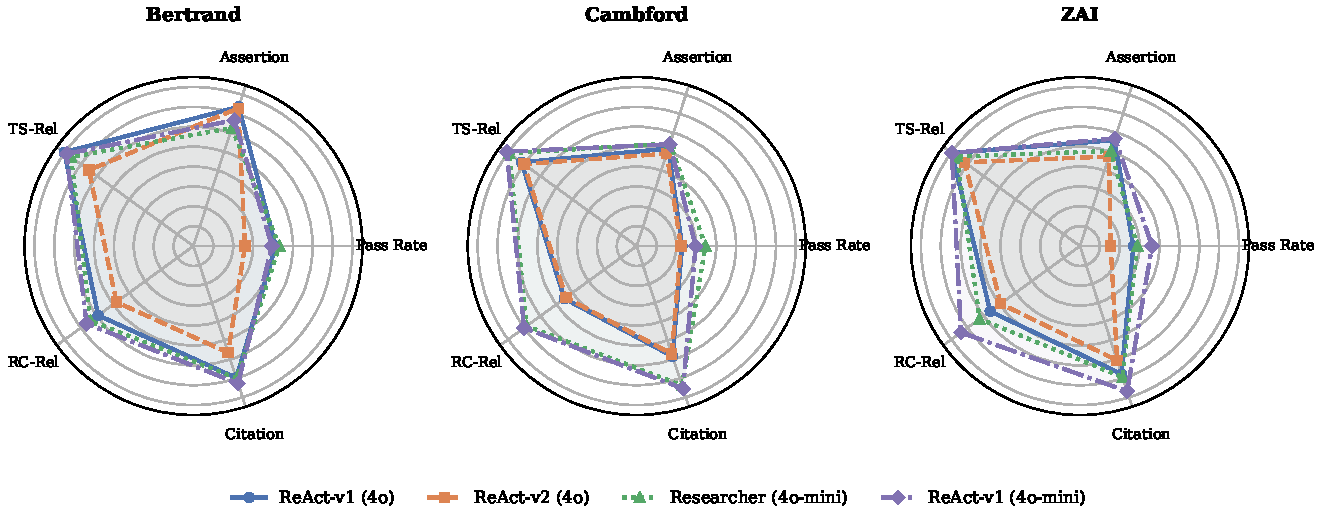
\includegraphics[width=\linewidth]{figures/agent_radar.pdf}
\caption{Per-tenant agent profiles. Each subplot shows the three agents on a shared radar for one tenant. On Bertrand (dense, small) all agents overlap; on Cambford (temporal multi-hop) \textsc{Researcher}'s citation and pass-rate advantage widens; on ZAI (large, bursty) \textsc{ReAct-v1} matches or exceeds the planner on assertion accuracy.}
\label{fig:agent_radar}
\end{figure}

\subsubsection{Query-Type Analysis}
\label{sec:query-type-analysis}

The evaluation set comprises three query categories generated with a 40/40/20 target split: \emph{fact-check} (single-entity retrieval), \emph{multi-hop} (cross-artifact reasoning), and \emph{report} (multi-source synthesis). Breaking down assertion and citation metrics by query type reveals how each architecture handles increasing retrieval complexity.

\begin{figure}[h]
\centering
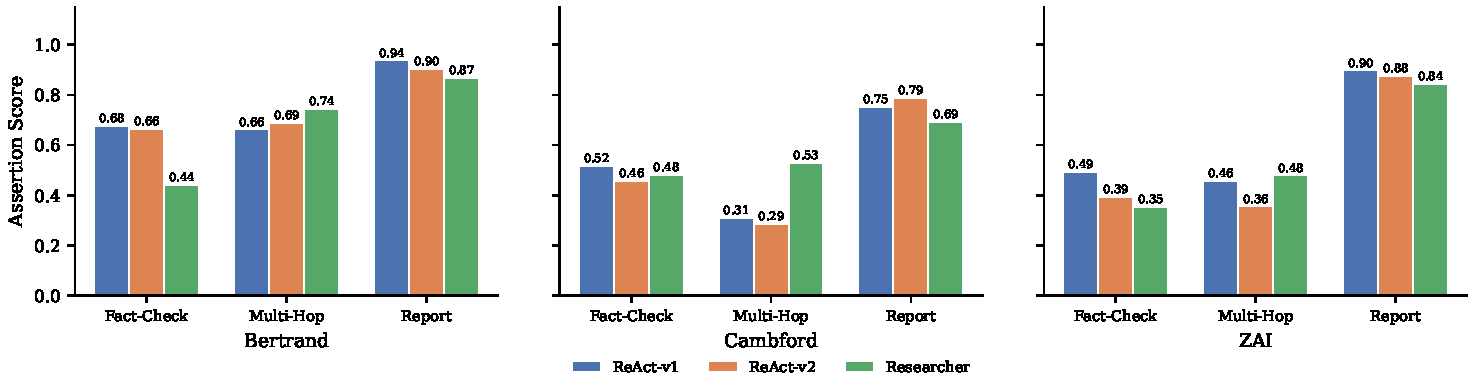
\includegraphics[width=\linewidth]{figures/assertion_by_query_type.pdf}
\caption{Mean assertion score by query type and tenant. All agents perform best on fact-check queries. The gap between agents widens on multi-hop and report queries, where \textsc{ReAct-v1}'s precision advantage is most pronounced.}
\label{fig:assertion_by_query_type}
\end{figure}

\begin{figure}[h]
\centering
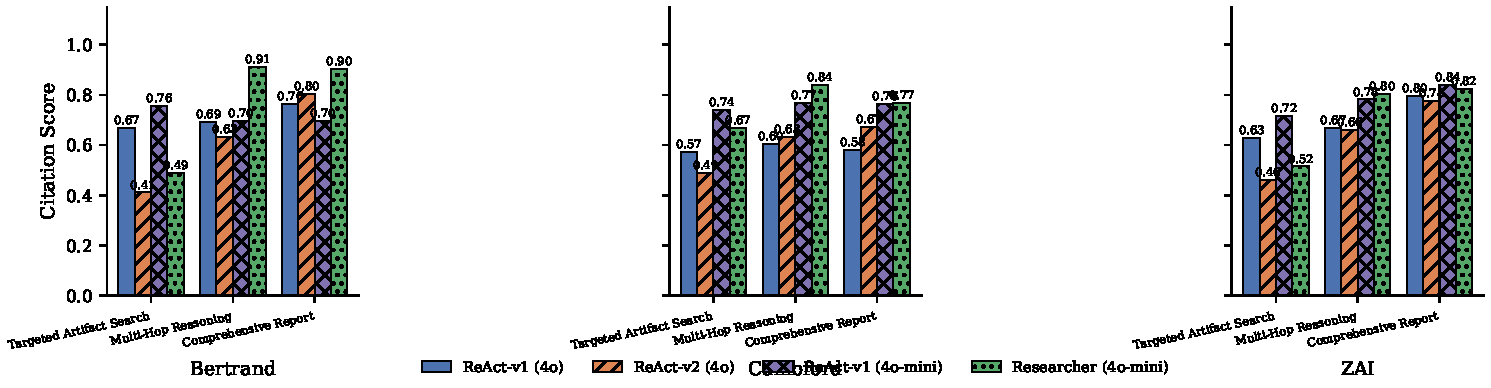
\includegraphics[width=\linewidth]{figures/citation_by_query_type.pdf}
\caption{Mean citation score by query type and tenant. \textsc{Researcher} leads on report queries where its planning stage systematically covers multiple source types, while the reactive agents are competitive on fact-check queries.}
\label{fig:citation_by_query_type}
\end{figure}

\begin{figure}[h]
\centering
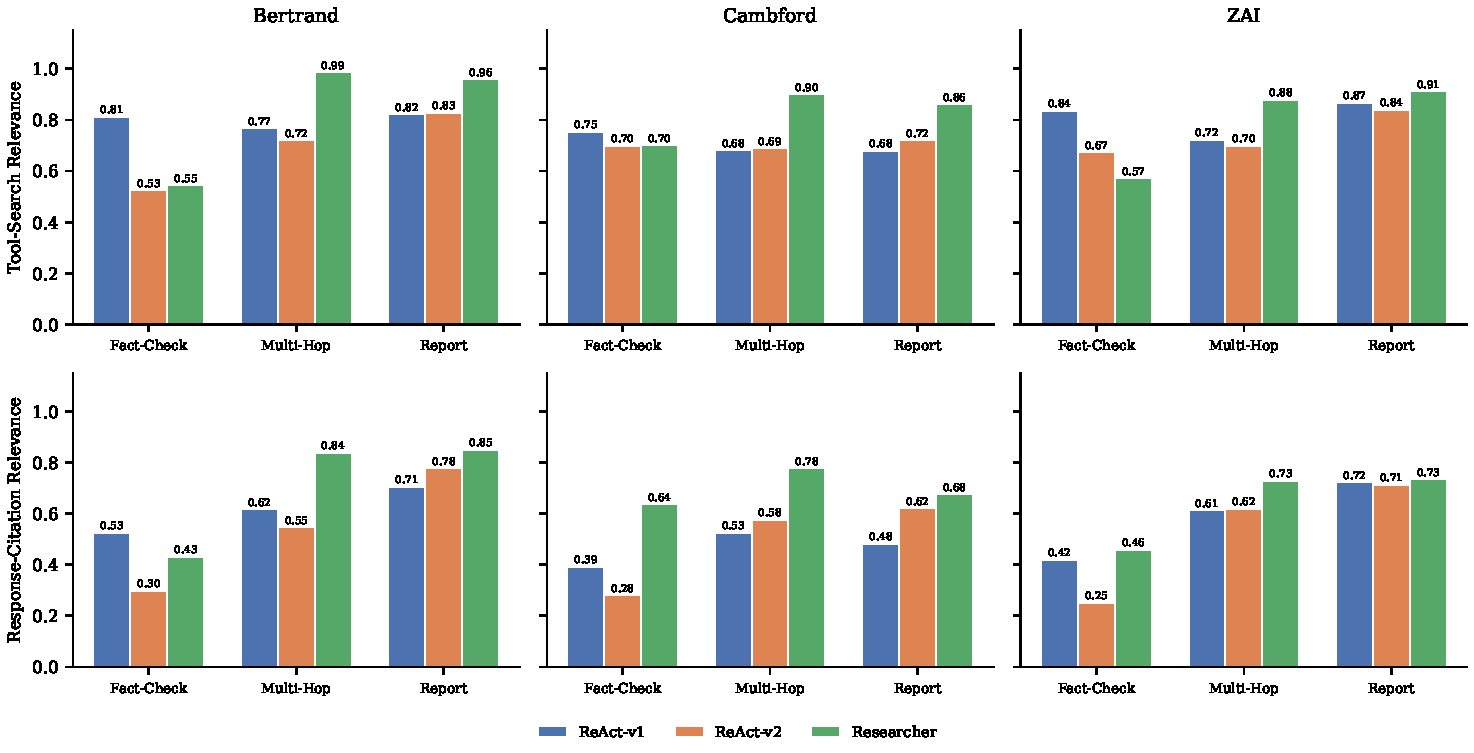
\includegraphics[width=\linewidth]{figures/citation_decomp_by_query_type.pdf}
\caption{Citation decomposition (tool-search relevance and response-citation relevance) by query type. Top row: tool-search relevance; bottom row: response-citation relevance. The performance gap between agents is most visible on report queries, where \textsc{Researcher}'s broader retrieval strategy produces higher relevance across both sub-metrics.}
\label{fig:citation_decomp_by_query_type}
\end{figure}

\noindent On fact-check queries, which require locating a single artifact, all three agents achieve their highest assertion scores and the inter-agent gap is narrow. This confirms that when evidence is concentrated in a single entity, even a minimal reactive loop suffices. On multi-hop queries, assertion scores drop across the board as agents must connect information across multiple artifacts; here \textsc{ReAct-v1}'s detailed worked examples help it maintain higher per-assertion accuracy than \textsc{Researcher}, whose broader retrieval introduces noise. On report queries, \textsc{Researcher}'s planning stage provides the clearest advantage in citation quality: its dependency-chain decomposition ensures that multiple source types are systematically retrieved and cited, while the reactive agents struggle to organize comprehensive responses from ad-hoc retrieval sequences.

\subsubsection{Cost–Effectiveness Trade-off}
\label{sec:cost-tradeoff}

The results reveal a clear cost-effectiveness frontier. \textsc{Researcher} achieves the highest pass rate (35.5\%) and citation quality (0.711) but consumes $5.2\times$ more prompt tokens (92{,}280 vs.\ 17{,}778) and $3.7\times$ more wall-clock time (65.2\,s vs.\ 17.6\,s) than~\textsc{ReAct-v1}. For deployments where retrieval completeness and citation traceability are the primary objectives---legal research, compliance auditing, or due-diligence workflows---this overhead may be justified. For latency-sensitive applications or scenarios with dense, recent evidence, \textsc{ReAct-v1} provides 32.3\% pass rate at $3.7\times$ lower latency with higher factual precision (assertion 0.638 vs.\ 0.557).

\textsc{ReAct-v2} does not occupy a Pareto-optimal point on this frontier: it matches \textsc{ReAct-v1} on tool-call count (1.70) and is marginally faster, but lags on all quality metrics. This finding suggests that prompt compression is costly in the absence of compensating architectural changes---a concise prompt is not equivalent to an equally effective one.

\begin{figure}[h]
\centering
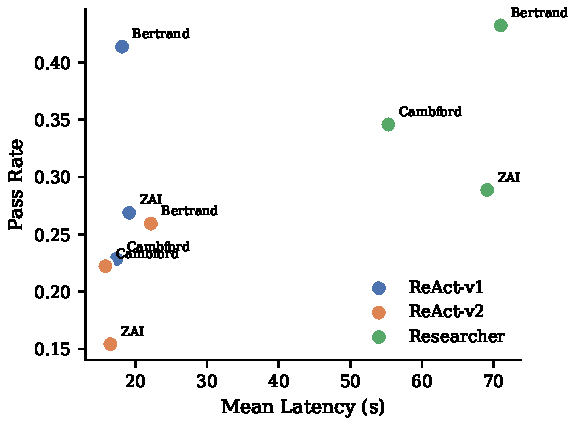
\includegraphics[width=0.75\linewidth]{figures/latency_vs_pass.pdf}
\caption{Latency--quality trade-off: mean wall-clock time vs.\ pass rate. \textsc{Researcher} occupies the high-latency/high-quality quadrant while the two reactive agents cluster at low latency; \textsc{ReAct-v1} achieves $3.7\times$ lower latency than \textsc{Researcher} with only a modest pass-rate gap.}
\label{fig:latency_vs_pass}
\end{figure}

\begin{figure}[h]
\centering
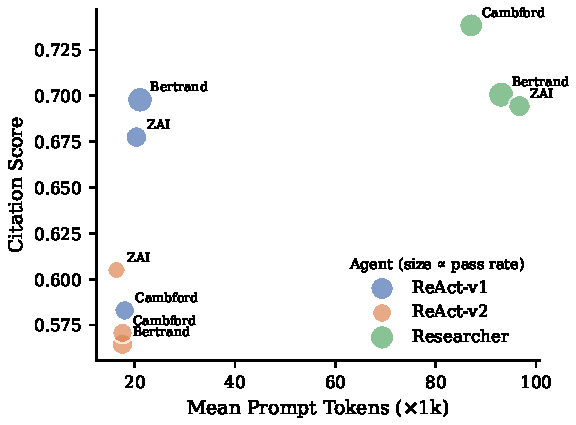
\includegraphics[width=0.7\linewidth]{figures/cost_quality_frontier.pdf}
\caption{Cost--quality frontier: mean prompt tokens vs.\ citation score. Marker size is proportional to pass rate. \textsc{Researcher} achieves the highest citation quality at $5.2\times$ the token cost of the reactive agents; \textsc{ReAct-v2} does not occupy a Pareto-optimal point.}
\label{fig:cost_frontier}
\end{figure}


\subsection{Cross-Model Evaluation and Bias Mitigation}
\label{sec:cross-model}

A synthetic benchmark must guard against circularity: if the same model family generates the data, runs the agent, and judges the output, self-preference bias can inflate scores. The EABench protocol treats the generator, runtime, and judge as three independent factors. In the experiments reported above, the generator and judge both use GPT-4o while the runtime varies across three agent configurations that differ in architecture, prompt design, and model size (GPT-4o for the ReAct agents, GPT-4o-mini for the Researcher). This setup reflects the realistic practitioner design space in which architecture, prompting, and model choice are varied jointly. To fully control for generator--judge bias, the framework supports a cross-model matrix in which tenants generated by model family $G_i$ are evaluated by runtime $R_j$ and judged by $J_k$, with the restriction that no conclusion is drawn from a single diagonal cell. Diagonal effects---where a model consistently scores higher only when generating or judging its own data---can then be identified as self-preference rather than genuine method improvement.

\subsection{Discussion}
\label{sec:exp-discussion}

The experiments expose three principal findings. First, the separation of planning from execution provides a measurable advantage on multi-hop temporal queries (52\% relative pass-rate improvement on Cambford) but negligible benefit on organizationally concentrated evidence (4\% improvement on Bertrand). This interaction between architecture and scenario structure is precisely the kind of diagnostic that a configurable benchmark is designed to surface. Second, prompt engineering matters as much as architecture: the 11-point pass-rate gap between \textsc{ReAct-v1} and \textsc{ReAct-v2}---identical architectures differing only in prompt verbosity and temperature---exceeds the 3-point gap between \textsc{ReAct-v1} and \textsc{Researcher} on two of three tenants. Third, the decomposed citation metrics reveal that retrieval quality and citation formatting are largely independent failure modes: \textsc{ReAct-v1} leads on tool-search relevance (0.799) while \textsc{Researcher} leads on response-citation quality (0.649), indicating that broad retrieval and well-structured references require different capabilities.

These findings suggest that future work should explore hybrid architectures that conditionally activate planning based on query complexity, as well as prompt-optimization techniques that maintain the behavioral specificity of verbose prompts at lower token cost.

% ══════════════════════════════════════════════════════════════════════
% 5  CONCLUSION AND DISCUSSION
% ══════════════════════════════════════════════════════════════════════
\section{Conclusion and Discussion}
\label{sec:conclusion}

\textcolor{blue}{EABench reframes enterprise-agent benchmarking as an end-to-end systems problem. Instead of providing only a fixed dataset or only a runtime abstraction, it joins four ingredients in a single platform: coherent tenant generation, configurable agent execution, configurable query and judge generation, and scenario-aware debugging under access control. This combination is what makes the benchmark useful for research rather than merely descriptive. It lets investigators ask not only whether one agent outperforms another, but why that difference appears and whether it survives changes in scenario, model family, retrieval stack, or judge configuration.}

\textcolor{blue}{The framework still has clear limitations. It currently assumes English-language enterprise communication, depends on sufficiently capable foundation models to preserve long-range narrative coherence during generation, and relies on judge prompts whose scope must be reviewed carefully when researchers introduce new task families. In addition, interactive debugging is a complement to formal evaluation rather than a substitute for it: visual inspection can diagnose failure modes, but final comparisons must still be grounded in reproducible case-level metrics.}

\textcolor{blue}{These limitations point directly to future work. The next priorities are broader multilingual support, richer sandbox backends for code-centric enterprise tasks, stronger controls against generator--judge self-preference bias, and expanded human validation protocols for both realism and scoring quality. Even in its current form, however, EABench provides a practical and extensible foundation for studying enterprise LLM agents under realistic data, realistic constraints, and experimentally meaningful variation.}

% ══════════════════════════════════════════════════════════════════════
% REFERENCES
% ══════════════════════════════════════════════════════════════════════
\bibliographystyle{ACM-Reference-Format}
\bibliography{bibliography}

\end{document}

















